% ------------------------------------------------------------------------------
% FORMAT TEMPLATE OF DOCUMENTATION / USER'S MANUAL
% ------------------------------------------------------------------------------


% DOCUMENT HEADER---------------------------------------------------------------
%   This template is based on "scrreprt" as part of the koma script.
% ------------------------------------------------------------------------------
\documentclass[
    11pt,      % font size
    DIV10,
    ngerman,   % language-specific package (umlauts, hyphenation etc.)
    textgreek,
    a4paper,   % paper size and format
    oneside,   % single-sided document
    titlepage, % usage of cover sheet
    parskip=half,          % spacing between paragraphs (half line)
    headings=normal,       % reduce size of captions
    listof=totoc,          % add lists to table of contents
    bibliography=totoc,    % add bibliography to table of contents
    index=totoc,           % add indices to table of contents
    captions=tableheading, % add annotations under figures 
    final                  % document's state (final/draft)
]{scrreprt}

% LANGUAGE OF DOCUMENT ---------------------------------------------------------
% Adjustment of the document's language ----------------------------------------
%\usepackage[english]{babel} 
\usepackage[ngerman]{babel}

% Here you can select the document's language. Any language-specific 
% part will be replaced. 
%\newcommand{\lang}{en}
\newcommand{\lang}{de}
% ------------------------------------------------------------------------------


% global Definitions -----------------------------------------------------------
%   meta-data of the document like title, author, date
%   are defined in global_defs.tex and can be used globally
% ------------------------------------------------------------------------------
% global_defs.tex -- en (English)
% Language specific file of ../global_defs.tex
%
% Here all language-specific global definitions are done



% the following \newcommands with German identifiers are necessary 
% when using the koma-script:
\newcommand{\titel}{Gaming Controller based on the {\Esplora} Board}      % title for header line and cover sheet
\newcommand{\untertitel}{}                                                % optionally a sub title
\newcommand{\Bezeichnung}{Esplora\-Gaming\-Con\-troller}                  % identifier, name of the topic
\newcommand{\Dokumentart}{U s e r ' s \ \ M a n u a l}                    % documentation type ("User's Manual", "Operating Instructions" etc.)
\newcommand{\autor}{schlizb�da}                                           % author

% other language-dependent elements
\newcommand{\publication}{date:\\Jan 31th, 2019}

% used hardware
\newcommand{\Esplora}{Arduino Esplora}
\newcommand{\RPi}{Raspberry Pi}


% used packages ----------------------------------------------------------------
%   used LaTeX packages are moved to the file packages.tex
%   to kkep this file tiny.
% ------------------------------------------------------------------------------
% Adjustment of page layout ----------------------------------------------------
%   see style.tex
% ------------------------------------------------------------------------------
\usepackage[
    automark, % Kapitelangaben in Kopfzeile automatisch erstellen
    headsepline, % Trennlinie unter Kopfzeile
    ilines % Trennlinie linksb�ndig ausrichten
]{scrpage2}

% Umlauts ----------------------------------------------------------------------
%   Set CodePage:
%   Use special characters like German umlauts (����)  directly in the LaTeX
%   source. Enables correct hyphenation rules for words containing umlauts.
% ------------------------------------------------------------------------------
\usepackage[latin1]{inputenc}
%\usepackage[utf8]{inputenc}
\usepackage[T1]{fontenc}
\usepackage{textcomp} % Euro char, Copyright etc.

% font -------------------------------------------------------------------------
\usepackage{lmodern} % better fonts
\usepackage{relsize} % Set relative font size

% Graphics and Pictures --------------------------------------------------------
% Enable including of JPG files
\usepackage[dvips,final]{graphicx}
% relative graphics path
\graphicspath{{pics/}}

% Commands from AMSTeX for mathematical symbols as \boldsymbol \mathbb ---------
\usepackage{amsmath,amsfonts}

% Index output with \printindex ------------------------------------------------
\usepackage{makeidx}

% Easy definition of line spacing, page margins etc. ---------------------------
\usepackage{setspace}
\usepackage{geometry}

% ------------------------------------------------------------------------------
% --- index of abbreviations ---------------------------------------------------
% ------------------------------------------------------------------------------
% Create symbol directories easily. Based on MakeIndex:
%  makeindex.exe %Name%.nlo -s nomencl.is -o %Name%.nls
% creates the directory. This command can be used e.g. in TeXnicCenter
% as a postprocessor, so that it needn't to be used manually all the time.
% The definitions are moved into the file "Glossar.tex".
% ------------------------------------------------------------------------------
\usepackage[intoc]{nomencl}
\let\abbrev\nomenclature
\renewcommand{\nomname}{Abk�rzungsverzeichnis}
\setlength{\nomlabelwidth}{.25\hsize}
\renewcommand{\nomlabel}[1]{#1 \dotfill}
\setlength{\nomitemsep}{-\parsep}

\usepackage{acronym}


% Text flow around images ------------------------------------------------------
\usepackage{floatflt}

% ------------------------------------------------------------------------------
% --- Listings to include source code ------------------------------------------
% ------------------------------------------------------------------------------
\usepackage{listings}
\usepackage[table]{xcolor} 
% colours for syntax colouring / alternatively: {RGB}{0-255,0-255.0-255}
%%%%\definecolor{hellgelb}{rgb}{1,1,0.9}			     
\definecolor{colKeys}{rgb}{0,0,1}
\definecolor{colIdentifier}{rgb}{0,0,0}
\definecolor{colComments}{rgb}{0,0.5,0.1} 
\definecolor{colString}{rgb}{1,0,0}
\lstset{
    float=hbp,
    basicstyle=\ttfamily\color{black}\small\smaller, % the size of the fonts that are used for the code 
    identifierstyle=\color{colIdentifier},
    keywordstyle=\color{colKeys},
    stringstyle=\color{colString},
    commentstyle=\color{colComments},
    columns=flexible,
    tabsize=3,
    %frame=single,                     % add frame arround the code
    extendedchars=true,
    showspaces=false,
    showstringspaces=false,
    numbers=left,                      % where to put the line numbers
    numberstyle=\tiny,                 % fontsize for line
    stepnumber= 1,                     % stepnumber between line-numbers
    breaklines=true,                   % sets automatic line breaking
    captionpos=b,                      % sets caption position to bottom
    backgroundcolor=\color{hellgelb},
    breakautoindent=true,
    }

% URL handling -----------------------------------------------------------------
\usepackage{url}

% important for correct citation -----------------------------------------------
\usepackage[numbers]{natbib}  % [square] to [numbers]

% ------------------------------------------------------------------------------
% --- PDF options --------------------------------------------------------------
% ------------------------------------------------------------------------------
\definecolor{darkblue}{rgb}{0,0,0.5} % colour of PDF links
\usepackage[
    bookmarks,
    bookmarksopen=true,
    colorlinks=true,
% colour definition of PDF links
    linkcolor=darkblue,% simple internal links
    anchorcolor=black, % anchor text
    citecolor=blue,    % links to bibliography
    filecolor=magenta, % links to open local files
    menucolor=red,     % Acrobat menu items
    urlcolor=cyan, 
% colour definitions for printing (all in black)
    %linkcolor=black,  % simple internal links
    %anchorcolor=black,% anchor text
    %citecolor=black,  % links to bibliography
    %filecolor=black,  % links to open local files
    %menucolor=black,  % Acrobat menu items
    %urlcolor=black, 
    backref,
    % for correct creation of bookmarks:
    plainpages=false,
    pdfpagelabels,
    hypertexnames=false,
    linktocpage % link to page numbers insteag of text
]{hyperref}
% Commands that output umlauts lead to errors when they are passed as options to hyperref
\hypersetup{
    pdftitle={\titel \untertitel},
    pdfauthor={\autor},
    pdfcreator={\autor},
    pdfsubject={\titel \untertitel},
    pdfkeywords={\titel \untertitel},
}

% Continuous Numbering of foot notes -------------------------------------------
\usepackage{chngcntr}

% for long tables --------------------------------------------------------------
\usepackage{longtable}
\usepackage{array}
\usepackage{ragged2e}
\usepackage{lscape}

% column definitions at right margin with defined width ------------------------
\newcolumntype{w}[1]{>{\raggedleft\hspace{0pt}}p{#1}}

% Change format of lists -------------------------------------------------------
\usepackage{paralist}

% necessary for definition of own commands
\usepackage{ifthen}

% defines commands for \todo and \listoftodos etc.
\usepackage{todonotes}

% ensures that spaces behind parameterless macros are not interpreted as macro end characters
\usepackage{xspace}

% format of figure annotations (captions)
\usepackage{caption}
\captionsetup{labelfont=bf,textfont=it} % figure bold, text italic

% including of message boxes
\usepackage[tikz]{bclogo}

% include underlining of text
\usepackage{ulem}

% format of tables
\usepackage{booktabs}
\renewcommand{\arraystretch}{1} % line spacing inside tables of 2

% including PDF files
\usepackage{pdfpages}


% activate creation of Index and list of abbreviations -------------------------
\makeindex
\makenomenclature

% Header, footer, page margins etc. --------------------------------------------


% Line spacing 1.5 lines -----------------------------------------------------
\onehalfspacing

% ------------------------------------------------------------------------------
% ----------- Page margins -----------------------------------------------------
% ------------------------------------------------------------------------------

\setlength{\topskip}{\ht\strutbox} % removes warnings from geometry
\geometry{paper=a4paper,left=30mm,right=25mm,top=20mm,bottom=40mm}
% additional binding offset (left margin)

% ------------------------------------------------------------------------------
% ----------- Headers and Footers ----------------------------------------------
% ------------------------------------------------------------------------------

\pagestyle{scrheadings}
% Header and footer even on initial chapter pages
\renewcommand*{\chapterpagestyle}{scrheadings} 
% Font of header line
\renewcommand{\headfont}{\normalfont}

%%% HEADER LINE %%%
\ihead{\hspace*{16pt} \large{\textsc{\titel}} \\[1ex] \textit{\hspace*{16pt} \headmark}}
\chead{}
%\ohead{\includegraphics[scale=0.06]{\logo}}
\setlength{\headheight}{21mm} % Height of header
% Widen the header beyond the text
\setheadwidth[-20pt]{textwithmarginpar} % negative values move to left side, 0=center
\setheadsepline[text]{0.4pt}[\hspace{20pt}] % Separator line below header

%%% FOOTER %%%
\ifoot{}  %\ifoot{\copyright\ \autor} add author optionally
\cfoot{- \pagemark ~-}
\ofoot{}

% ------------------------------------------------------------------------------
% ----------- other typographical settings -------------------------------------
% ------------------------------------------------------------------------------

\frenchspacing % Creates a little bit more space after a full stop

% avoid orphan lines and widow lines
\clubpenalty = 10000
\widowpenalty = 10000 
\displaywidowpenalty = 10000

% Format source code output (listings?)
\lstset{numbers=left, numberstyle=\tiny, numbersep=5pt, breaklines=true}
\lstset{emph={square}, emphstyle=\color{red}, emph={[2]root,base}, emphstyle={[2]\color{blue}}}

% continuous numbering of foot notes
\counterwithout{footnote}{chapter}

%\parindent 0pt % no insertion after NewLine


% own LaTeX commands
% Own commands and typographic styles for this documentation
% ------------------------------------------------------------------------------

% easy change of font e.g.: \changefont{cmss}{sbc}{n}
\newcommand{\changefont}[3]{\fontfamily{#1} \fontseries{#2} \fontshape{#3} \selectfont}

% ------------------------------------------------------------------------------
% Abbreviations with correct typographic space
%-------------------------------------------------------------------------------
% Own commands and typographic styles for this documentation
% ------------------------------------------------------------------------------

% easy change of font e.g.: \changefont{cmss}{sbc}{n}
\newcommand{\changefont}[3]{\fontfamily{#1} \fontseries{#2} \fontshape{#3} \selectfont}

% ------------------------------------------------------------------------------
% Abbreviations with correct typographic space
%-------------------------------------------------------------------------------
% Own commands and typographic styles for this documentation
% ------------------------------------------------------------------------------

% easy change of font e.g.: \changefont{cmss}{sbc}{n}
\newcommand{\changefont}[3]{\fontfamily{#1} \fontseries{#2} \fontshape{#3} \selectfont}

% ------------------------------------------------------------------------------
% Abbreviations with correct typographic space
%-------------------------------------------------------------------------------
\input{layout/\lang/commands} % language-specific text line



\newcommand{\bs}{$\backslash$}

% Creates a list element with bold caption
\newcommand{\itemd}[2]{\item{\textbf{#1}}\\{#2}}

%% -----------------------------------------------------------------------------
%% some commands concerning to citation
%% -----------------------------------------------------------------------------
%\newcommand{\Zitat}[2][\empty]{\ifthenelse{\equal{#1}{\empty}}{\citep{#2}}{\citep[#1]{#2}}}
%
%% printing of authors
%\newcommand{\AutorName}[1]{\textsc{#1}}
%\newcommand{\Autor}[1]{\AutorName{\citeauthor{#1}}}
%
%% -----------------------------------------------------------------------------
%% various commands to semantically mark words
%% -----------------------------------------------------------------------------
%\newcommand{\NeuerBegriff}[1]{\textbf{#1}}
%\newcommand{\Fachbegriff}[1]{\textit{#1}}
%
%\newcommand{\Eingabe}[1]{\texttt{#1}}
%\newcommand{\Code}[1]{\texttt{#1}}
%\newcommand{\Datei}[1]{\texttt{#1}}
%
%\newcommand{\Datentyp}[1]{\textsf{#1}}
%\newcommand{\XMLElement}[1]{\textsf{#1}}
%\newcommand{\Webservice}[1]{\textsf{#1}}
%
 % language-specific text line



\newcommand{\bs}{$\backslash$}

% Creates a list element with bold caption
\newcommand{\itemd}[2]{\item{\textbf{#1}}\\{#2}}

%% -----------------------------------------------------------------------------
%% some commands concerning to citation
%% -----------------------------------------------------------------------------
%\newcommand{\Zitat}[2][\empty]{\ifthenelse{\equal{#1}{\empty}}{\citep{#2}}{\citep[#1]{#2}}}
%
%% printing of authors
%\newcommand{\AutorName}[1]{\textsc{#1}}
%\newcommand{\Autor}[1]{\AutorName{\citeauthor{#1}}}
%
%% -----------------------------------------------------------------------------
%% various commands to semantically mark words
%% -----------------------------------------------------------------------------
%\newcommand{\NeuerBegriff}[1]{\textbf{#1}}
%\newcommand{\Fachbegriff}[1]{\textit{#1}}
%
%\newcommand{\Eingabe}[1]{\texttt{#1}}
%\newcommand{\Code}[1]{\texttt{#1}}
%\newcommand{\Datei}[1]{\texttt{#1}}
%
%\newcommand{\Datentyp}[1]{\textsf{#1}}
%\newcommand{\XMLElement}[1]{\textsf{#1}}
%\newcommand{\Webservice}[1]{\textsf{#1}}
%
 % language-specific text line



\newcommand{\bs}{$\backslash$}

% Creates a list element with bold caption
\newcommand{\itemd}[2]{\item{\textbf{#1}}\\{#2}}

%% -----------------------------------------------------------------------------
%% some commands concerning to citation
%% -----------------------------------------------------------------------------
%\newcommand{\Zitat}[2][\empty]{\ifthenelse{\equal{#1}{\empty}}{\citep{#2}}{\citep[#1]{#2}}}
%
%% printing of authors
%\newcommand{\AutorName}[1]{\textsc{#1}}
%\newcommand{\Autor}[1]{\AutorName{\citeauthor{#1}}}
%
%% -----------------------------------------------------------------------------
%% various commands to semantically mark words
%% -----------------------------------------------------------------------------
%\newcommand{\NeuerBegriff}[1]{\textbf{#1}}
%\newcommand{\Fachbegriff}[1]{\textit{#1}}
%
%\newcommand{\Eingabe}[1]{\texttt{#1}}
%\newcommand{\Code}[1]{\texttt{#1}}
%\newcommand{\Datei}[1]{\texttt{#1}}
%
%\newcommand{\Datentyp}[1]{\textsf{#1}}
%\newcommand{\XMLElement}[1]{\textsf{#1}}
%\newcommand{\Webservice}[1]{\textsf{#1}}
%


% DOCUMENT ---------------------------------------------------------------------
%   The contents of the document starts here.
%   Parts of the document are moved to external files. 
%   Here these files will be included.
% ------------------------------------------------------------------------------
% ------------------------------------------------------------------------------
\begin{document}

% enumberation of subsubsections
\setcounter{secnumdepth}{3}
\setcounter{tocdepth}{3}

% Page numbering ---------------------------------------------------------------
%   Prefaces are numbered pages are numbered in capital Roman numerals.
% ------------------------------------------------------------------------------
%%%%\pagenumbering{Roman} % I dislike this!
\pagenumbering{arabic}    % Take arabic numbers everywhere

% cover sheet and abstract without page numbering
\cfoot{}
% coversheet.tex -- en (English)
% Language specific file of ../coversheet.tex
%
% This file contains language-specific texts.
\center{This document was created using the typesetting system \LaTeX{}}

%\include{layout/abstract}
\cfoot{- \pagemark ~-}

\tableofcontents   % table of contents
\listoffigures     % list of figures
\listoftables      % list of tables
\renewcommand{\lstlistlistingname}{Verzeichnis der Listings}
%\lstlistoflistings % list of source code listings

%% list of abbreviations -------------------------------------------------------
%\input{Kapitel/Glossar}
%% for correct caption in the header line
%\clearpage\markboth{\nomname}{\nomname} 
%\printnomenclature
%\label{sec:Glossar}


% arabic page numbers in the main part -----------------------------------------
%%%%\clearpage
%%%%\pagenumbering{arabic}


% ##############################################################################
% ----------   including of chapters   -----------------------------------------
% ##############################################################################
% chapter1.tex -- de (German)
\chapter{Einleitung}

Vielen Dank f�r Ihr Interesse an {\autor}s {\Bezeichnung}.\\
Hierbei handelt es sich um ein Steuerger�t f�r PCs, das Tastatur- und
Mausaktionen emulieren kann und den Steuerger�ten (Gaming Controllern)
der diversen Spielekonsolen nachempfunden ist. Es basiert auf dem 
Arduino-Board \textit{Esplora}, das technisch einem \textit{Arduino 
Leonardo} entspricht, aber bereits einige Sensoren und Aktoren enth�lt
und dessen Leiterplatte grob die Form eines Gaming Controllers aufweist.

\url{https://store.arduino.cc/arduino-esplora}

\section{Rechtliche Hinweise}
Bei der Konzeption des {\Bezeichnung}s wurde darauf geachtet, nur
Software zu verwenden, die unter einer freien Lizenz wie GNU GPL oder
�hnlichem zur Verf�gung gestellt wird oder ganz in die 
\textit{Gemeinfreiheit} (engl. \textit{public domain}) entlassen wurde.

\subsection*{Marken}
Einige Bezeichnungen in dieser Schrift k�nnen Marken sein, deren
Benutzung durch Dritte f�r deren Zwecke die Rechte der Inhaber verletzen
k�nnen.

\subsection*{Links}
In dieser Bedienungsanleitung sind Links zu externen Seiten im Internet 
enthalten. Diese Inhalte macht sich der Verfasser {\autor} trotz
Verlinkung nicht zu eigen, da sie nicht in seinem Einflussbereich
stehen! Zum Zeitpunkt der Verlinkung waren keine rechtswidrigen Inhalte
erkennnbar. Eine st�ndige �berpr�fung auf etwaige rechtsversto�ende
�nderungen ist dem Verfasser nach geltendem Recht nicht zuzumuten.\\
Sollten aktuelle oder k�nftige Inhalte jedoch rechtswidrig sein, so kann
der Autor dar�ber per e-mail an \url{mailto:himself@schlizbaeda.de}
informiert werden. Es werden dann entsprechende Ma�nahmen zur
Beseitigung des/der betroffenen Links ergriffen.

\subsection*{Lizensierung der Bestandteile des Projektes}
\uline{Code:}\\
Die meisten Code-Beispiele werden von Arduino in die Gemeinfreiheit 
(\textit{public domain}) gestellt und k�nnen daher von jeder Person
verwendet werden. Auch der Code f�r den {\Bezeichnung} wurde aus den
Codevorlagen\\
\url{https://www.arduino.cc/en/Tutorial/EsploraJoystickMouse},\\
\url{https://www.arduino.cc/en/Tutorial/EsploraKart} und\\
\url{https://github.com/circuit69/EsploraTinkerkit}\\
entwicket. Aufgrund zahlreicher Weiterentwicklungen und Anpassungen
beschloss der Autor jedoch, sein Werk unter der GNU GPL v3 zu
ver�ffentlichen:\\
\url{https://www.gnu.org/licenses/gpl-3.0.en.html}\\

\includegraphics[height=35px]{GPLv3.png}

\uline{Geh�use:}\\
Bei der Internetsuche nach einem passenden Geh�use wurde schlie�lich auf
\\ \url{https://www.thingiverse.com/thing:45880} ein Satz Dateien f�r
einen 3D-Druck gefunden, der unter CC BY-NC 3.0 
(\url{http://creativecommons.org/licenses/by-nc/3.0/}) lizensiert ist,
also keine kommerzielle Nutzung gestattet.\\

\includegraphics[height=35px]{CC-BY-NC.png}


\subsection*{Bildrechte}
Alle inhaltlich relevanten Fotos und technischen Abbildungen in diesem
Dokument stammen vom Verfasser {\autor} selbst und werden hiermit von
ihm unter der \textit{Creative-Commons}-Li\-zenz \textbf{CC BY-SA 3.0}
ver�ffentlicht. Sie d�rfen daher von jedem bei Namensnennung des 
Urhebers in unver�nderter oder auch in ver�nderter Form unter den 
gleichen Bedingungen weitergegeben werden:\\

\includegraphics[height=35px]{CC-BY-SA.png}

Das in dieser Dokumentation verwendete Arduino-Logo ist gemeinfrei:\\

\includegraphics[height=35px]{arduino.png}


\section{Hinweis zur neumodernen "`Genderei"' landauf, landab}
Der Autor {\autor} kann gar nicht oft genug betonen, dass ihm eine
Gleichbehandlung \textbf{aller} Geschlechter (mittlerweile mehr als 
zwei) �u�erst wichtig ist. Er verurteilt eine Diskriminierung von
Menschen nur aufgrund ihres Geschlechtes oder anderer
Nebens�chlichkeiten wie ihrer Herkunft etc. aufs Sch�rfste!

Dennoch -- oder gerade deswegen -- lehnt er die derzeit grassierende
Unart des sogenannten "`Genderns"' mit sprachlichen Ausw�chsen wie 
"`AnwenderInnen"' oder gar "`Benutzer*innen"' (jetzt neu mit Stern!)
zugunsten  einer klaren und verst�ndlichen Ausdrucksweise ab. In diesem
Trend sind selbst W�rter wie "`Abiturienten"' verp�nt: Soll man hier
wirklich gender-gerecht "`Abitu\-rierende"' schreiben? \smiley{wink}


\section{Danksagung}
{\autor} m�chte dem Benutzer \textbf{@dale}
(\url{https://forum-raspberrypi.de/user/23726-dale/}) aus dem deutschen
Raspberry Pi Forum (\url{https://forum-raspberrypi.de}) seinen Dank 
aussprechen: Er erkl�rte sich freundlicherweise bereit, das 
Esplora-Geh�use von \url{https://www.thingiverse.com} mit seinem 
3D-Drucker auszudrucken.


\section{Kurzbeschreibung}
Der {\Bezeichnung} ist ein den Gaming Controllern der g�ngigen 
Spielekonsolen nachempfundenes Steuerger�t mit USB-Anschluss. Anstelle
von propriet�ren Signalen �bermittelt dieses Ger�t bei Bet�tigung der
Bedienelemente entsprechende Tastatur- \bzw Mauskommandos, um damit die
laufende Software auf dem Computer zu steuern, an dem es �ber USB2.0
angeschlossen ist.

Aufgrund seiner quelloffenen und freien Programmierung kann es auf
beliebige Anwendungen/Szenarien angepasst werden, indem \textit{im 
Quellcode} den einzelnen Bedienelementen (Sensoren) die gew�nschten
Tastaturcodes oder Mauskommandos zugeordnet werden.

Es k�nnen acht verschiedene Belegungen f�r unterschiedliche
Anwendungsf�lle hinterlegt werden, die im laufenden Betrieb umgeschaltet
werden k�nnen. Die gew�hlte Einstellung wird �ber die Farbe der auf dem
Esplora-Board verbauten dreifarbigen LED angezeigt.

Softwareseitig emuliert der {\Bezeichnung} eine USB-Tastatur und eine
USB-Maus und kann auf den meisten PC-Betriebssystemen (Windows, 
GNU/Linux) sowie auf einem {\RPi} unter Raspbian sofort ohne
Treiberinstallation verwendet werden.

% chapter2.tex -- en (English)
\chapter{Operating Instructions}
\label{cha:manual}
This chapter is a classical operator's guide for users who intend to use
the {\Bezeichnung} straight forward without modifying the software or
hardware of the device.

\section{Controls of {\Bezeichnung}}
\begin{figure}[h]
\centering
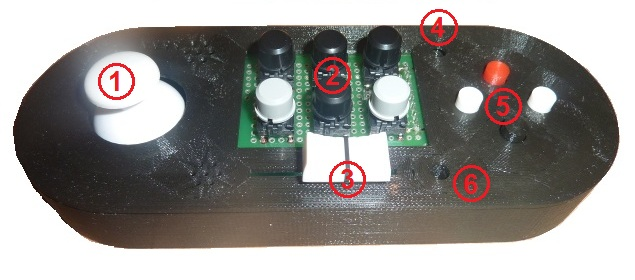
\includegraphics[width=0.8\textwidth]{controls_labeled.jpg}
\caption{Controls (Sensors) of {\Bezeichnung}}
\label{fig:controls}
\end{figure}

The listed controls of {\Bezeichnung} emulate keyboard and mouse:

\begin{table}[h]
\centering
\renewcommand{\arraystretch}{1.5}
\begin{tabular}{|p{0.05\textwidth}|p{0.25\textwidth}|p{0.60\textwidth}|}
\hline
\textbf{num.}		&	\textbf{Element}	&	\textbf{Function}\\
\hline
		1)			&	joystick			&	mouse movement\\
\hline
		2)			&	TinkerKit switches	&	mouse buttons, keyboard\\
\hline
		3)			&	slider				&	mouse scroll wheel\\
\hline
		4)			&	light sensor		&	\textit{usually disabled}\\
\hline
		5)			&	cursor pushbuttons	&	cursor key codes\\
\hline
		6)			&	three-colour LED	&	shows the selected assignment\\
\hline
\end{tabular}
\vspace{0.5cm}
\caption{Controls (Sensors) of {\Bezeichnung}}
\end{table}

\subsection*{Joystick}
The joystick usually emulates mouse movements. Depending on the
displacement of the joystick, the speed of the mouse movement is
adjusted. Pressing the joystick emulates a click on the left mouse
button.\\
On the Esplora board, the joystick is converted by two potentiometers,
whose position is read via A/D converters of the built-in 8-bit ATMEL
microcontroller \textit{ATmega32U4}. When the joystick is pressed, a
push button is actuated which is digitally read.

\subsection*{TinkerKit Switches}
On the {\Bezeichnung} there is a small additional printed circuit board
at the place where a small display would actually be installed. On this
additional board there are six pushbuttons, which are connected to the
four TinkerKit connectors. The white TinkerKit connectors are
implemented as analogue inputs, so that a sophisticated voltage divider
combination can be used to differentiate which key combination is
pressed.\\
These six buttons are assigned to additional keyboard codes or mouse
clicks.

\subsection*{Slider}
The slider control is a potentiometer connected to an A/D converter of 
the ATMEL microcontroller. It usually emulates the scrolling wheel of
the mouse.\\
Of course simply releasing the slider is not sufficient to stop the
emulated scrolling wheel! Rather, the controller must be pushed a little
bit in the opposite direction to stop the scrolling process.

\subsection*{Light Sensor}
The light sensor is connected to another A/D converter of the ATMEL
microcontroller. Some tests of the light sensor showed quickly that it
cannot be implemented as a kind of actuator. Even lightweight shadowing
will result in missinterpretations. Nevertheless the Arduino sketch
still contains some software routines to implement a control element.
However, the light sensor is disabled in most assignment modes.

\subsection*{Cursor Pushbuttons}
These four pushbuttons are digitally read by the ATMEL microcontroller.
They emulate keyboard codes to control the cursor or for moving a game
character by emulating the keys A, W, S and D. Many computer
games expect these keys.

\subsection*{Three-coloured LED}
The three-coloured LED shows the selected controller assignment (mode)
by changing its colour. See section \ref{sect:assignment}

\section{Selecting the Assignment Mode of the Actuators}
\label{sect:assignment}
Pressing all four cursor pushbuttons simultaneously starts the
setting mode of the {\Bezeichnung}. Using the UP and DOWN pushbuttons
will change the assignment of the acutators. The colour of the
three-colour LED changes according to the currently selected
assignment.\\
By pressing all four cursor pushbuttons simultaneously again, the
setting mode of the device will be quit. To prevent accidental changes
of the selected assignment mode, it is recommended to start with
pressing the cursor pushbutton LEFT or RIGHT and then pressing the
others.

\begin{table}[h]
\centering
\renewcommand{\arraystretch}{1.5}
\begin{tabular}{|p{0.05\textwidth}|p{0.15\textwidth}|p{0.70\textwidth}|}
\hline
\textbf{num.}		&	\textbf{LED colour}		&	\textbf{denomination}\\
\hline
		0)			&	\textit{``dark white''}	&	common 1\\
\hline
		1)			&	red						&	MinecraftPi\\
\hline
		2)			&	green					&	yamuplay \textit{t.b.d. (to be defined)}\\
\hline
		3)			&	yellow					&	<<undefined 3>>\\
\hline
		4)			&	blue					&	<<undefined 4>>\\
\hline
		5)			&	magenta					&	<<undefined 5>>\\
\hline
		6)			&	cyan					&	<<undefined 6>>\\
\hline
		7)			&	white					&	common 2\\
\hline
\end{tabular}
\vspace{0.5cm}
\caption{The Eight Assignment Modes for the Actuators of \Bezeichnung}
\end{table}
 
\uline{\textbf{common 1: } LED: ``dark white'' (low light emission)}\\
In this assignment mode the actuators emulate solely keyboard codes. No
mouse functions are used.

\begin{tabular}{ll}
	joystick			&	cursor keys\\
	joystick pushbutton	&	ENTER key\\
	slider				&	Pg-up, pg-dn\\
	light sensor		&	\textit{inactive}\\
	TinkerKit orange	&	SPACE key, ESC key\\
	TinkerKit white		&	modifier keys SHIFT, CTRL, ALT\\
\end{tabular}

	
\uline{\textbf{MinecraftPi: } LED: red}\\
The assignment is adapted for the game \textit{MinecraftPi} for the
\RPi.

\begin{tabular}{ll}
	joystick			&	mouse movement (to adjust the viewing angle)\\
	joystick pushbutton	&	key \texttt{E} to open the Minecraft block select menu\\
	slider				&	mouse scrolling wheel for quick block selection\\
	light sensor		&	\textit{inactive}\\
	TinkerKit orange	&	left and right mouse button\\
	TinkerKit white		&	keys ENTER, SHIFT, ESC, SPACE\\
\end{tabular}
	
	
\uline{\textbf{yamuplay: } LED: green}\\
Here it is planned to implement an assignment for controlling 
{\autor}'s media player \textit{yamuplay.py}.\\
\url{https://github.com/schlizbaeda/yamuplay}

Currently this is an undefined assignment mode!

\uline{\textbf{<<undefined 3>>: } LED: yellow}\\
This is an undefined assignment mode!

\uline{\textbf{<<undefined 4>>: } LED: blue}\\
This is an undefined assignment mode!

\uline{\textbf{<<undefined 5>>: } LED: magenta}\\
This is an undefined assignment mode!

\uline{\textbf{<<undefined 6>>: } LED: cyan}\\
This is an undefined assignment mode!

\uline{\textbf{common 2: } LED: white}\\
This mode emulates keyboard and mouse actions.

\begin{tabular}{ll}
	joystick			&	mouse movement\\
	joystick pushbutton	&	left mouse button\\
	slider				&	mouse scrolling wheel\\
	light sensor		&	\textit{inactive}\\
	TinkerKit orange	&	left and right mouse button\\
	TinkerKit white		&	modifier keys SHIFT, CTRL, ALT\\
\end{tabular}

% chapter3.tex -- de (German)
\chapter{�nderung am \Bezeichnung}

In diesem Kapitel wird die Herangehensweise f�r �nderungen an diesem
Projekt beschrieben:\\
Der Hardwareteil beschreibt in erster Linie den Einbau der erg�nzten
Zusatzleiterplatte mit den Tastern f�r die TinkerKit-Anschl�sse.\\
F�r den Softwareteil wird vorausgesetzt, dass der Leser die Arduino-IDE
erfolgreich auf seinem PC installiert hat und wei�, wie eine
Arduino-Baugruppe damit programmiert wird.

\section{Beschreibung der Zusatzplatine f�r die TinkerKit-Taster}
\label{sect:TinkerKitBoard}
Moderne Gaming Controller haben in der Regel mehr als nur die vier
Cursortasten. Meist sind sogenannte Schultertasten an der Vorderkante
des Controllers verbaut, die direkt mit den Zeigefingern bedient werden
k�nnen.

Beim {\Bezeichnung} werden die vier TinkerKit-Anschl�sse verwendet, um
weitere Taster hinzuzuf�gen. Da die wei�en TinkerKit-Anschl�sse auf
Pins des \textit{ATmega32U4}-Mikrocontrollers verdrahtet sind, die �ber
einen 10bit A/D-Wandler eingelesen werden, k�nnen pro wei�em
TinkerKit-Anschluss mehrere Taster �ber entsprechende Spannungsteiler
\textbf{gleichzeitig} betrieben und unterschieden werden.
%In Abbildung \ref{fig:fritzing} ist die Verdrahtung der Tasten an den
%TinkerKit-Anschl�ssen dargestellt.
%
%\begin{figure}[!h]
%\centering
%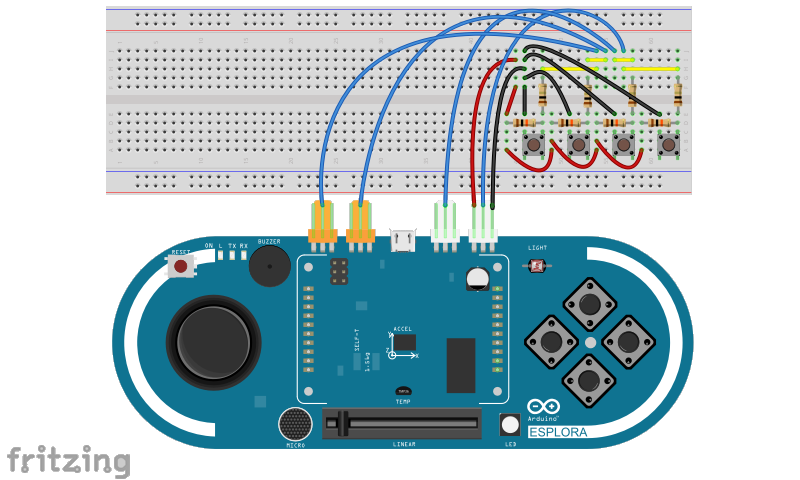
\includegraphics[width=0.8\textwidth]{fritzing.png}
%\caption{Verdrahtung der TinkerKit-Anschl�sse}
%\label{fig:fritzing}
%\end{figure}

Auf dem ersten Prototypen der Zusatzplatine wurden an jedem analogen
TinkerKit-Anschluss (wei�) jeweils zwei Taster mit den Spannungsteilern
33k : 22k \bzw 33k : 47k angeschlossen. Dies resultiert in folgenden
Spannungen und A/D-Werten:

\begin{table}[h]
\centering
\renewcommand{\arraystretch}{1.5}
\begin{tabular}{p{0.20\textwidth}p{0.20\textwidth}p{0.20\textwidth}}
	\textbf{Taster}	&	\textbf{A/D-Wert}	&	\textbf{Spannung}\\
	kein Taster		&	1023				&	5,00V\\
	47k-Taster		&	601					&	2,94V\\
	22k-Taster		&	410					&	2,00V\\
	beide Taster	&	320					&	1,56V\\
\end{tabular}
\vspace{0.5cm}
\caption{A/D-Werte der TinkerKit-Taster}
\end{table}

Die folgenden Bilder zeigen den Anschluss des Prototyps. Im Anhang ist
das Schaltungskonzept sowie eine Leiterplatte dargestellt, die bis zu
sechs Taster an den wei�en TinkerKit-Anschl�ssen erm�glichen.
 
\newpage
\begin{figure}[!h]
\centering
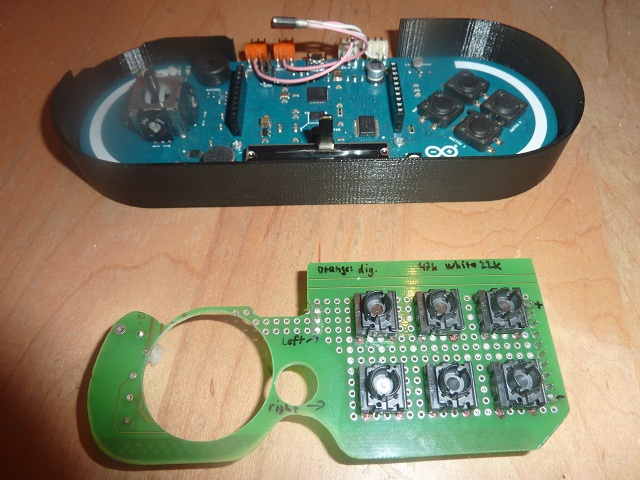
\includegraphics[width=0.85\textwidth]{esplora01.jpg}
\caption{Arduino Esplora und TinkerKit-Zusatzplatine (Prototyp)}
\label{fig:esplora01}
\end{figure}

\begin{figure}[!h]
\centering
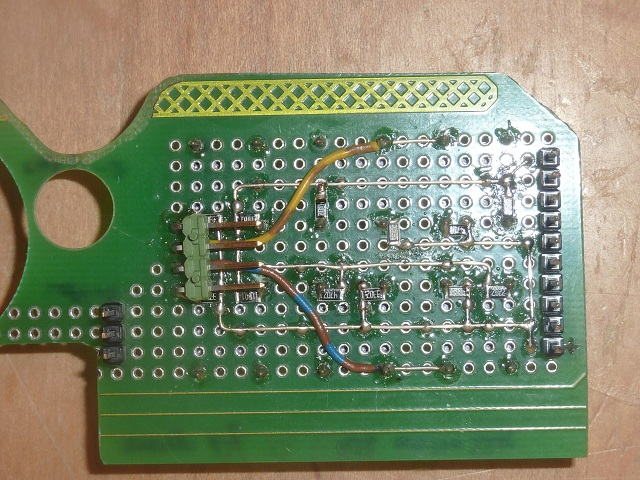
\includegraphics[width=0.85\textwidth]{esplora02.jpg}
\caption{Widerst�nde der TinkerKit-Zusatzplatine}
\label{fig:esplora02}
\end{figure}

\newpage
\begin{figure}[!h]
\centering
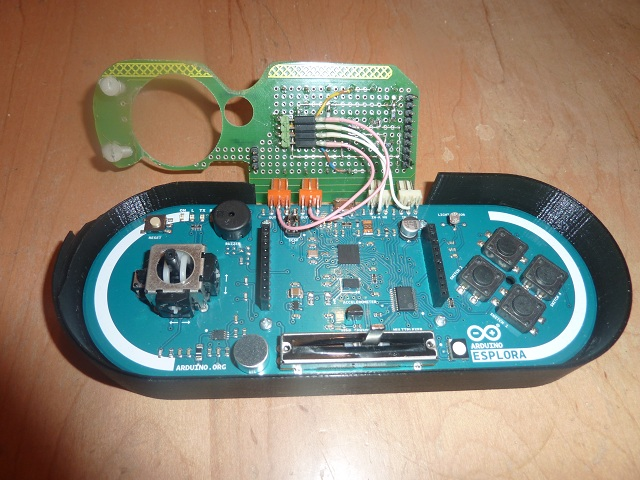
\includegraphics[width=0.85\textwidth]{esplora03.jpg}
\caption{Anschluss der TinkerKit-Zusatzplatine am Arduino Esplora}
\label{fig:esplora03}
\end{figure}

\begin{figure}[!h]
\centering
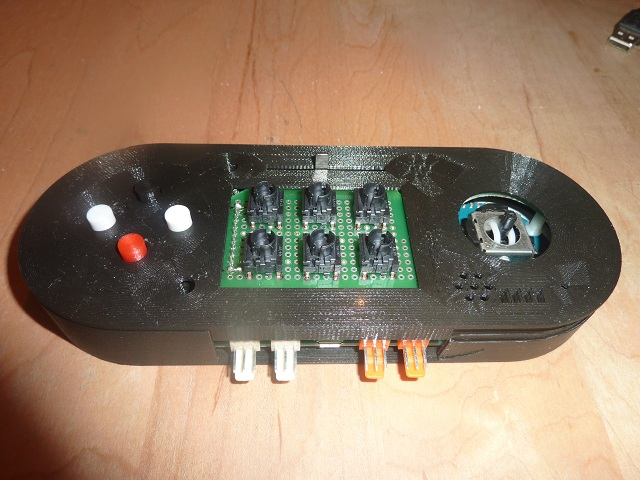
\includegraphics[width=0.85\textwidth]{esplora04.jpg}
\caption{TinkerKit-Zusatzplatine eingebaut}
\label{fig:esplora04}
\end{figure}



\newpage
\section{Beschreibung des Arduino-Sketch f�r den \Bezeichnung}
\subsection{Installation der Arduino-IDE}
Eine vollst�ndige Beschreibung zur Inbetriebnahme des \textit{Arduino
Web Editors} oder der \textit{Arduino Desktop IDE} findet sich auf der
Internetseite \url{https://www.arduino.cc/en/Guide/HomePage}. Dabei
sollte sich jeder Anwender nach eigenem Gusto f�r eine Variante
entscheiden.

\subsection{Anpassung des Codes}
Ein Arduino Esplora Board, das mit dem heruntegeladenen Sketch 
\texttt{EsploraGamingController.ino} programmiert wird, emuliert eine
USB-Maus und eine USB-Tastatur, wie in Kapitel \ref{cha:manual} 
beschrieben.

Die einfachste Art, den Code anzupassen, ist, die Werte der
zweidimensionalen Arrayvariablen \texttt{gl\_modeKeycodes} den eigenen
W�nschen gem�� abzu�ndern und das Arduino Esplora Board neu zu flashen.
Eine Liste der Tastaturcodes f�r nicht-ASCII-Zeichen befindet sich in
der Datei \texttt{Esplora\_ExtendedKeycodes.txt}.\\
Der Wert 0 bedeutet dabei, dass die im Code vorgesehene
\textbf{Mausbelegung} f�r das entsprechende Bedienelement verwendet
wird:
\begin{table}[h]
\centering
\renewcommand{\arraystretch}{1.5}
\begin{tabular}{|p{0.25\textwidth}|p{0.70\textwidth}|}
\hline
\textbf{Bedienelement}	&	\textbf{Mausbelegung bei Wert 0}\\
\hline
	Joystickbewegung	&	Mausbewegung\\
\hline
	Joystick Druck		&	Linksklick\\
\hline
	TinkerKit orange	&	Linksklick, Rechtsklick\\
\hline
	TinkerKit wei�		&	\textbf{keine Mausfunktionalit�t!}\\
\hline
	Schieberegler		&	Scrollrad\\
\hline
	Helligkeitssensor	&	Rechtsklick\\
\hline
	Cursortasten		&	\textbf{keine Mausfunktionalit�t!}\\
\hline
\end{tabular}
\vspace{0.5cm}
\caption{Standardmausbelegungen der Bedienelemente}
\end{table}

Um ein Bedienelement ganz zu deaktivieren, muss ihm der Wert 255 (\bzw
die Konstante \texttt{FUNCT\_DISABLED}) zugewiesen werden.

Die analogen Bedienelemente liefern einen Wert zwischen 0 und 1023, da
sie �ber einen 10-bit A/D-Wandler eingelesen werden. Beim Joystick
bestimmen die ausgelesenen 10-bit-Werte die Geschwindigkeit der
Mausbewegung. Gleiches gilt bei der Definition von Tastaturcodes f�r den
Joystick: Hier wird die Wiederholrate der entsprechenden Taste ebenfalls
von der Joystickauslenkung bestimmt.\\
Der Schieberegler emuliert die Drehung des Scrollrades der Maus. Auch
hier bestimmt die Auslenkung die Geschwindigkeit der Scrollbefehle. Um
das Scrolling zu stoppen, muss der Schieberegler nur leicht zur�ck in
Richtung Mitte geschoben werden. Dies funktioniert sogar dann, wenn der
ausgelesene Wert an sich ein Scrolling bewirken w�rde. Relevant ist hier
das leichte Zur�ckschieben des Reglers.\\
Bei den wei�en TinkerKit-Tasten wird der Analogeingang daf�r verwendet,
eine Kombination aus jeweils zwei Tasten pro TinkerKit-Anschluss zu
ermitteln. Dies wird auf der Zusatzleiterplatte durch eine passende
Kombination von Spannungsteilern erm�glicht. Die Genzwerte sind in der
Arrayvariablen \texttt{TINKERKIT\_LEVEL} definiert. Dabei ist darauf zu
achten, dass die angegebenen Grenzwerte die Mittelwerte der jeweiligen
Tastendrucke sind, um eine sichere Auswertung zu gew�hrleisten.\\
Der Helligkeitssensor liefert ebenfalls einen 10-bit-Wert. Allerdings
kann er nur schwer f�r Bet�tigungsaktionen verwendet werden: Bereits
kleine �nderungen der Beleuchtungsverh�ltnisse, die durch versehentliche
Abdeckung des Sensors oder Drehen des ganzen Controllers verursacht
werden, f�hren zu fehlerhaften Aktionen. Daher wird empfohlen, den
Helligkeitssensor nicht zu verwenden und zu deaktivieren.

\subsection{Aufbau des Codes}
In diesem Abschnitt wird auf die wichtigsten \texttt{\#define}s,
Variablen und Funktionen des Quellcodes eingegangen:

\subsubsection*{serielle Schnittstelle (UART)}
Dieser Sketch emuliert neben Tastatur und Maus auch eine
USB-Schnitt\-stelle mit der Baud\-rate 9600. Unter Windows ist diese
serielle Schnittstelle im Ger�te-Manager als \textit{\textbf{COM<x>}}
sichtbar, unter GNU/Linux als \texttt{/dev/ttyACM<x>}. \todo{UART 
vern�nftig umsetzen}Derzeit sind die Daten, die �ber diese serielle
Schnittstelle zum PC gesendet werden, noch nicht sauber strukturiert!

\subsubsection*{\texttt{\#define}}
\uline{\texttt{\#define SERIAL\_DEBUG}}\\
Aktivieren/Deaktivieren von Debugmeldungen �ber die serielle
Schnittstelle.

\uline{\texttt{\#define LOOP\_DELAY}}\\
Legt die Wartezeit bei jedem Durchlauf in Millisekunden fest. Je kleiner
dieser Wert ist, umso schneller reagiert das Arduino Esplora Board auf
die �nderungen. Dies macht sich vor allem bei der Geschwindigkeit des
Mauszeigers aufgrund von Joystickbewegungen bemerkbar.\\
Zu kurze Zeiten wirken sich aufgrund prellender Tasten m�glicherweise 
negativ auf das Verhalten des Boards aus: Gedr�ckte Tasten werden dann
mitunter doppelt ausgef�hrt!

\subsubsection*{Variablen}
\uline{Variable \texttt{byte gl\_mode}}\\
Enth�lt die aktuell ausgew�hlte Belegung als Zahlenwert zwischen 0 und
7.

\uline{Arrayvariable \texttt{char* gl\_modeNames[8]}}\\
Hier sind Bezeichnungen f�r die acht unterschiedlichen Belegungen
hinterlegt. Diese Strings werden bei der Auswahl �ber die serielle
Schnittstelle ausgegeben.

\uline{zweidimensionale Arrayvariable \texttt{char gl\_modeKeycodes[8][18]}}\\
Hier werden die Tastatur- / Mauskommandos f�r die einzelnen
Bedienelemente eingetragen:\\
\begin{tabular}{ll}
0		&	Mauskommando\\
1-254	&	Tastaturkommando\\
255		&	deaktiviert\\
\end{tabular}

\subsubsection*{Funktionen}
\uline{Funktion \texttt{void setup()}}\\
Dies ist eine Standardfunktion eines Arduino-Sketches, die �ber die
Arduino-Bibliothek eingebunden wird. Sie wird zu Beginn einmalig
ausgef�hrt: Initialisierung der Variablen und Kalibrierung der analogen
Sensoren, insbesondere des Joysticks.

\uline{Funktion \texttt{void loop()}}\\
Dies ist eine Standardfunktion eines Arduino-Sketches, die �ber die
Arduino-Bibliothek eingebunden wird. Sie wird nach \texttt{setup()}
wiederholt in einer Endlosschleife aufgerufen und dient dem Pollen der
Sensoren der Bedienelemente.

\uline{Funktion \texttt{void setMode(byte mode)}}\\
W�hlt die angegebene Belegung (0-7) aus:
\begin{compactitem}
	\item{Setzt die Variable \texttt{gl\_mode} auf den parametrierten Wert}
	\item{Setzt die Farbe der dreifarbigen LED}
	\item{gibt die Bezeichnung der parametrierten Belegung �ber die serielle Schnittstelle aus.}
\end{compactitem}

\uline{Funktion \texttt{unsigned int readTinkerkitInput(byte whichInput)}}\\
Einlesen der TinkerKit-Eing�nge �ber Aufruf der Funktion
\texttt{readChannel(byte channel)}.

\uline{Funktion \texttt{unsigned int readChannel(byte channel)}}\\
Diese Funktion �berschreibt die gleichlautende Funktion in der
Arduino-Library \texttt{Esplora}. Das Auslesen der TinkerKit-Signale
erfolgt �ber einen Multiplexer-Chip auf dem Arduino Esplora Board.

\uline{Funktion \texttt{byte tinkerkitWhiteSwitches(unsigned int analogue)}}\\
Auswertung der gedr�ckten Tastenkombination an den wei�en
TinkerKit-Anschl�ssen. Hier ist die Variable \texttt{const unsigned int
TINKERKIT\_LEVEL[4]} definiert, in der die analogen Grenzwerte f�r die
Tastenkombinationen hinterlegt werden. Man findet diese Grenzwerte am
besten heraus, indem man diese Funktion mit allen Tastenkombinationen
aufruft und die Messwerte �ber die serielle Schnittstelle ausgibt. Diese
Messwerte sollten ziemlich genau in der Mitte zwischen zwei in dieser 
Arrayvariablen hinterlegten Grenzwerten liegen. Oder andersherum
gedacht, sollten die Grenzwerte in der Mitte der Messwerte von zwei
"`benachbarten"' Tastenkombinationen liegen.\\
Damit diese Funktion vern�nftig funktionieren kann, m�ssen die
Widerst�nde f�r die Spannungsteiler auf der Zusatzleiterplatte richtig
dimensioniert worden sein!

\section{Ausblick auf geplante Erweiterungen}
\begin{enumerate}
\item{�nderung der Tastenbelegung durch den Anwender �ber das Ger�t
      selbst,\\ohne Programmierung �ber die Arduino IDE}
\item{Speichern der Tastenbelegung im EEPROM des \textit{ATmega32U4}}
\item{Definition mehrerer Tastaturbefehle als Sequenz pro Sensor}
\item{Definition von Werten f�r bestimmte Mausaktionen}
\item{vern�nftige Ausgaben f�r die serielle Schnittstelle festlegen}
\end{enumerate}


% ##############################################################################
% ------------------------------------------------------------------------------
% ##############################################################################




% APPENDIX ---------------------------------------------------------------------
%   The contents of the appendix are included similar to the chapters.
%   This is done in the file appendix.tex
%   %%%% Page numbering is done with small Roman numerals.
% ------------------------------------------------------------------------------
\begin{appendix}
    \clearpage
%%%%    \pagenumbering{roman}
    \chapter{Anhang}
    \label{sec:appendix}
    % Adjust enumberation margin in tables
    \setdefaultleftmargin{1em}{}{}{}{}{}
    % appendix.tex -- de (German)
Der Anhang enth�lt die EAGLE-Zeichnungen zur TinkerKit-Zusatzplatine:
\begin{compactitem}
	\item Verdrahtungskonzept der TinkerKit-Taster
	\item Schaltplan der TinkerKit-Zusatzplatine
	\item Leiterplatte
	\begin{compactitem}
		\item Abmessungen
		\item Oberseite
		\item Unterseite
	\end{compactitem}
%	\item Best�ckung
\end{compactitem}

\section{Best�ckvarianten}
Die Leiterplatte kann so best�ckt werden, dass sie funktional dem in
Abschnitt \ref{sect:TinkerKitBoard} beschriebenen Prototypen
entspricht.\\
Alternativ kann die Best�ckung f�r sechs �ber Spannungsteiler
unterscheidbare Taster an den analogen Eing�ngen der wei�en 
TinkerKit-Anschl�sse ausgef�hrt werden. Die Taster f�r die digitalen
TinkerKit-Anschl�sse (orange) k�nnen an anderer Stelle (\zB als
Schultertasten am Geh�use) verbaut werden und an der Stiftleiste X1
angeschlossen werden.

Die gew�nschte Version kann �ber die dazugeh�rige Best�ckvariante aus
Tabelle \ref{tab:variants} festgelegt werden:

\begin{table}[h]
\centering
\renewcommand{\arraystretch}{1.5}
\begin{tabular}{|p{0.23\textwidth}|p{0.16\textwidth}|p{0.18\textwidth}|p{0.15\textwidth}|p{0.16\textwidth}|}
\hline
\textbf{Version}								&	\textbf{RDIG\_ORL, RDIG\_ORR}	&	\textbf{RANA\_ORL, RANA\_ORR}	&	\textbf{RDN\_ORL, RDN\_ORR}	&	\textbf{RDN\_PINL, RDN\_PINR}\\
\hline
	vier analoge Taster,\newline zwei digitale Taster	&	0R								&	nicht best�ckt					&	1k							&	nicht best�ckt\\
\hline
	sechs analoge Taster,\newline zwei externe Taster	&	nicht best�ckt					&	0R								&	68k oder 82k (t.b.d.)		&	1k\\
\hline
\end{tabular}
\vspace{0.5cm}
\caption{Best�ckvarianten}
\label{tab:variants}
\end{table}




%---------------------------------------------------------------
%  conception
%---------------------------------------------------------------
%%%%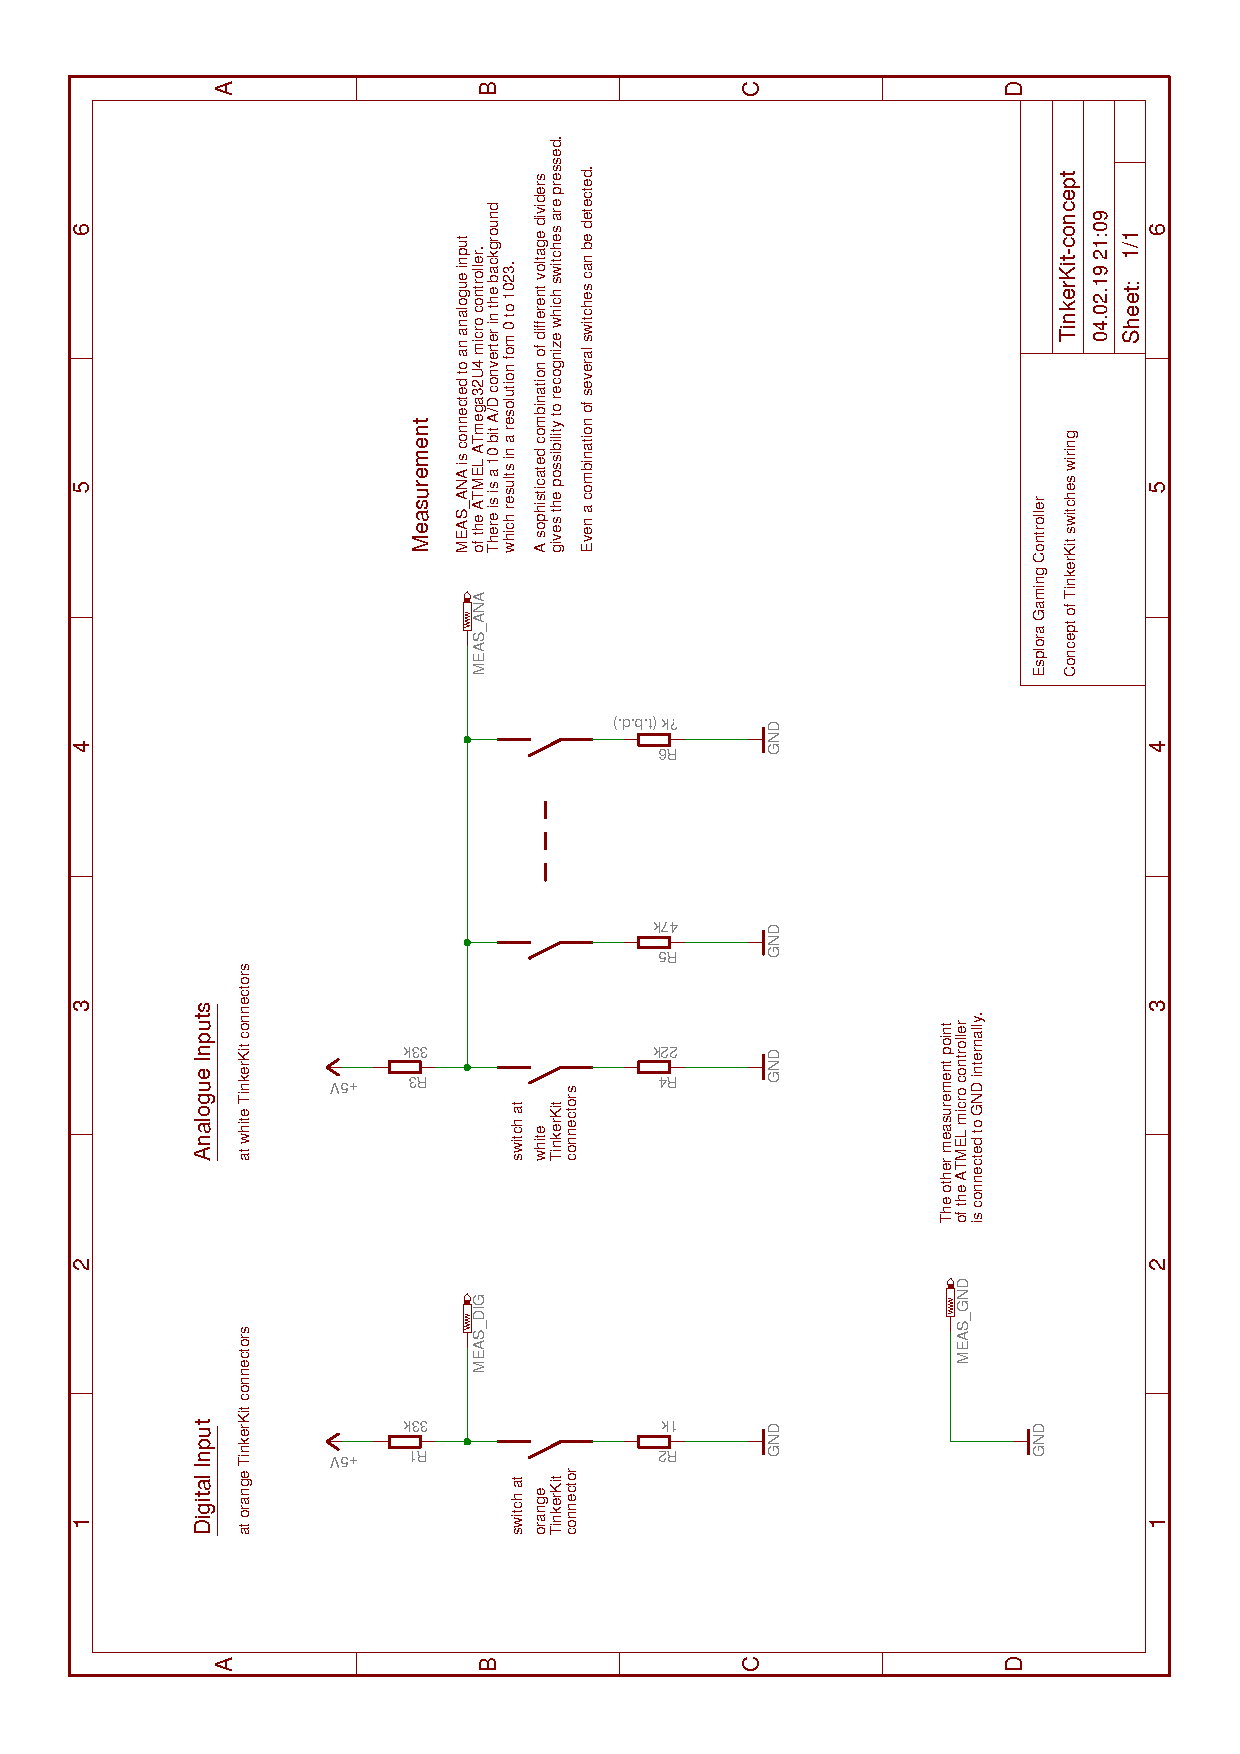
\includepdf[pages=-, portrait, scale=1.0, addtotoc={1,section,0,Konzept,Konzept} ]{./pics/eagle/TinkerKit-concept.pdf}
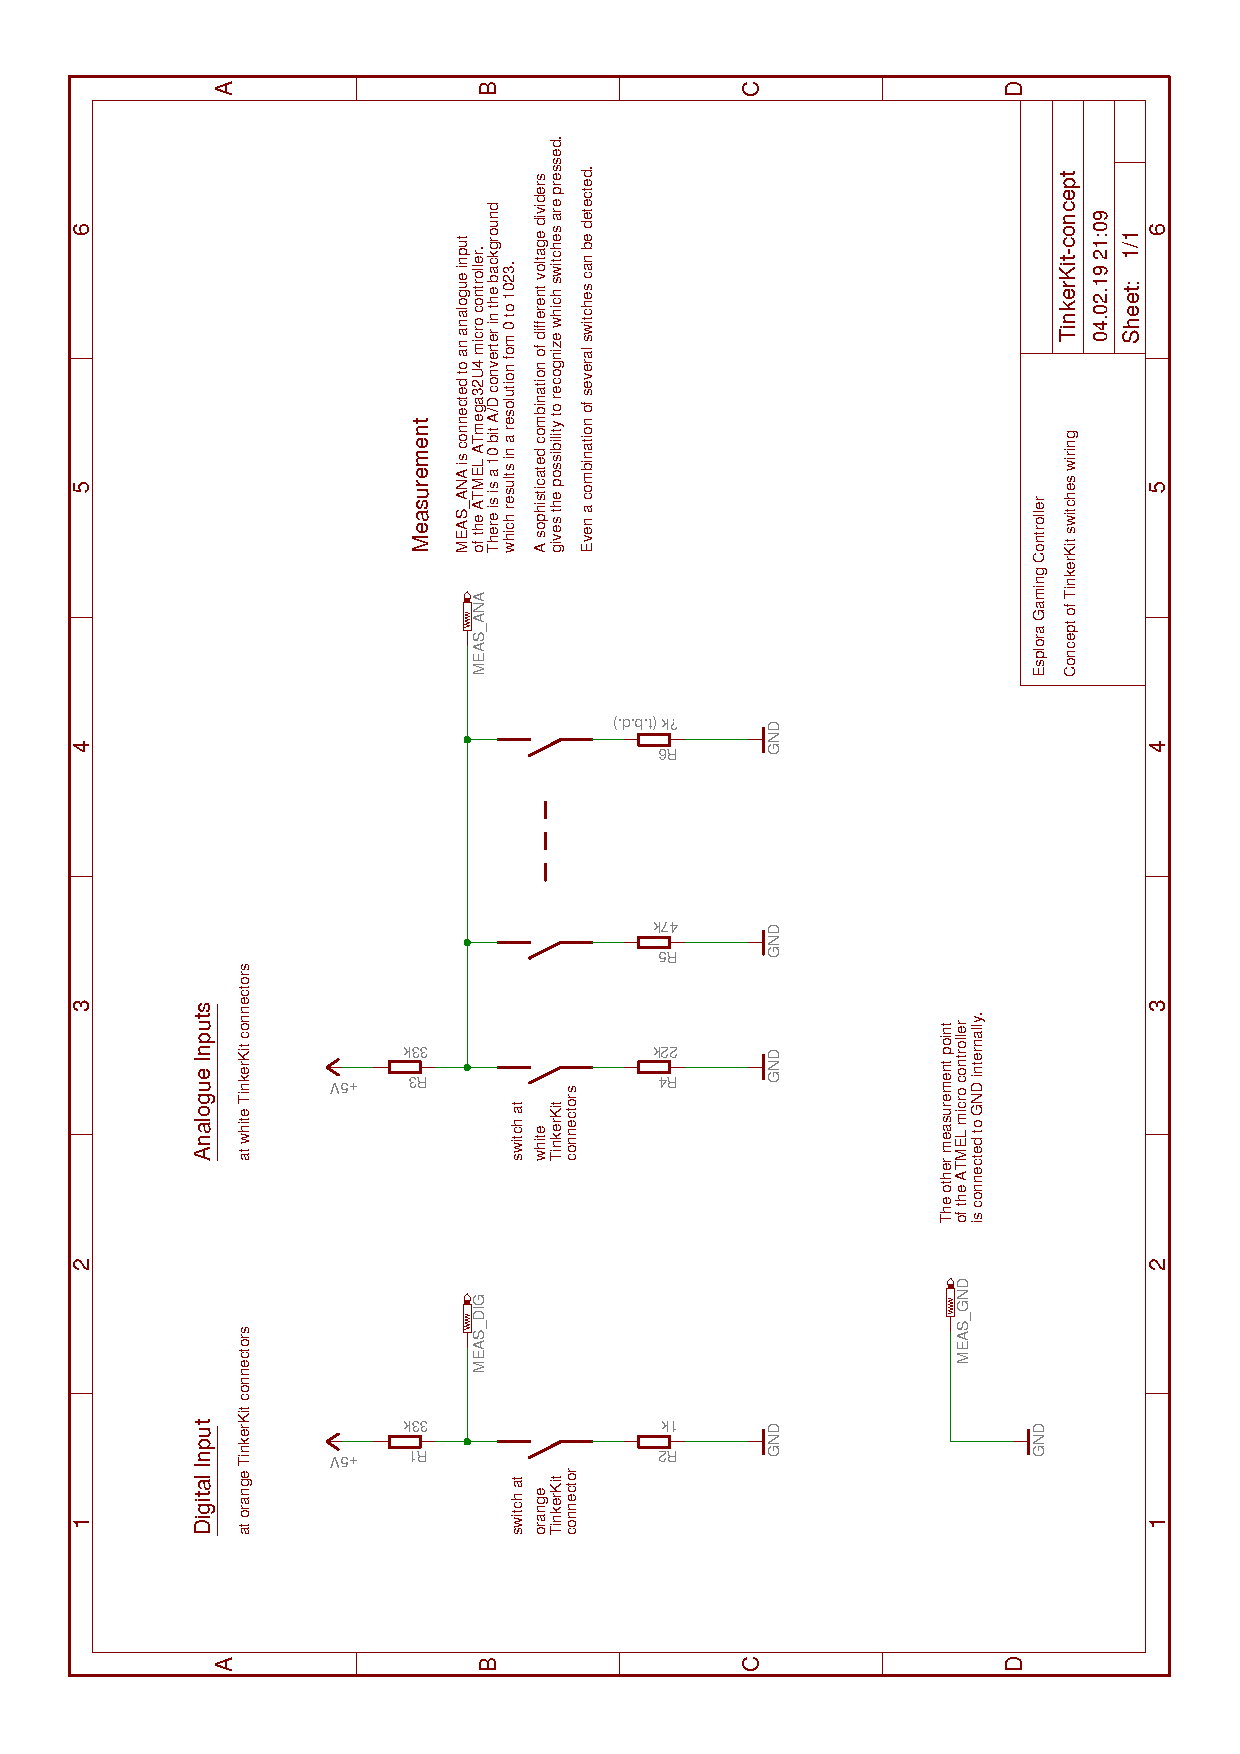
\includepdf[pages=-, , scale=1.0, addtotoc={1,section,0,Konzept,Konzept} ]{./pics/eagle/TinkerKit-concept.pdf}

%---------------------------------------------------------------
%  schematics
%---------------------------------------------------------------
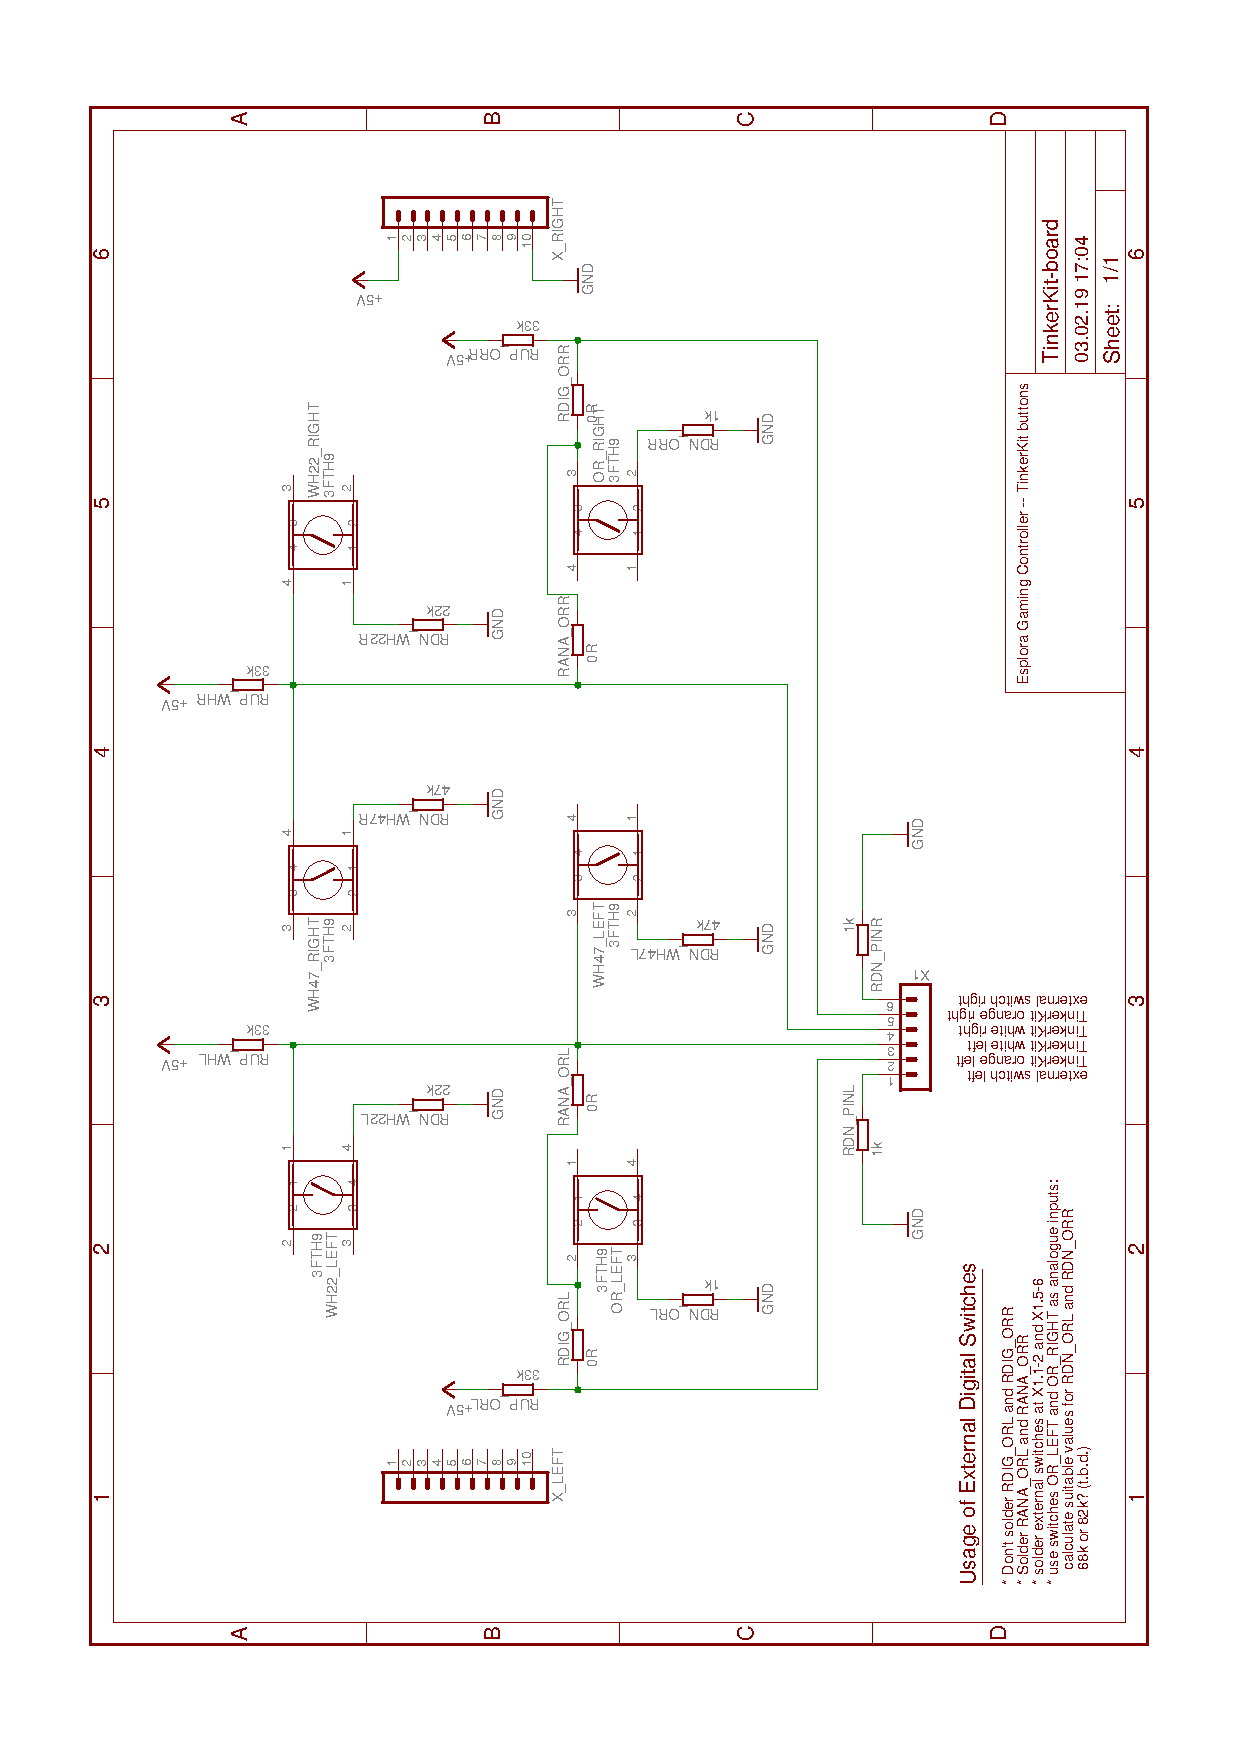
\includepdf[pages=-, , scale=1.0, addtotoc={1,section,0,Zusatzplatine Schaltplan,Zusatzplatine Schaltplan} ]{./pics/eagle/TinkerKit-board_SCH.pdf}

%---------------------------------------------------------------
%  PCB
%---------------------------------------------------------------
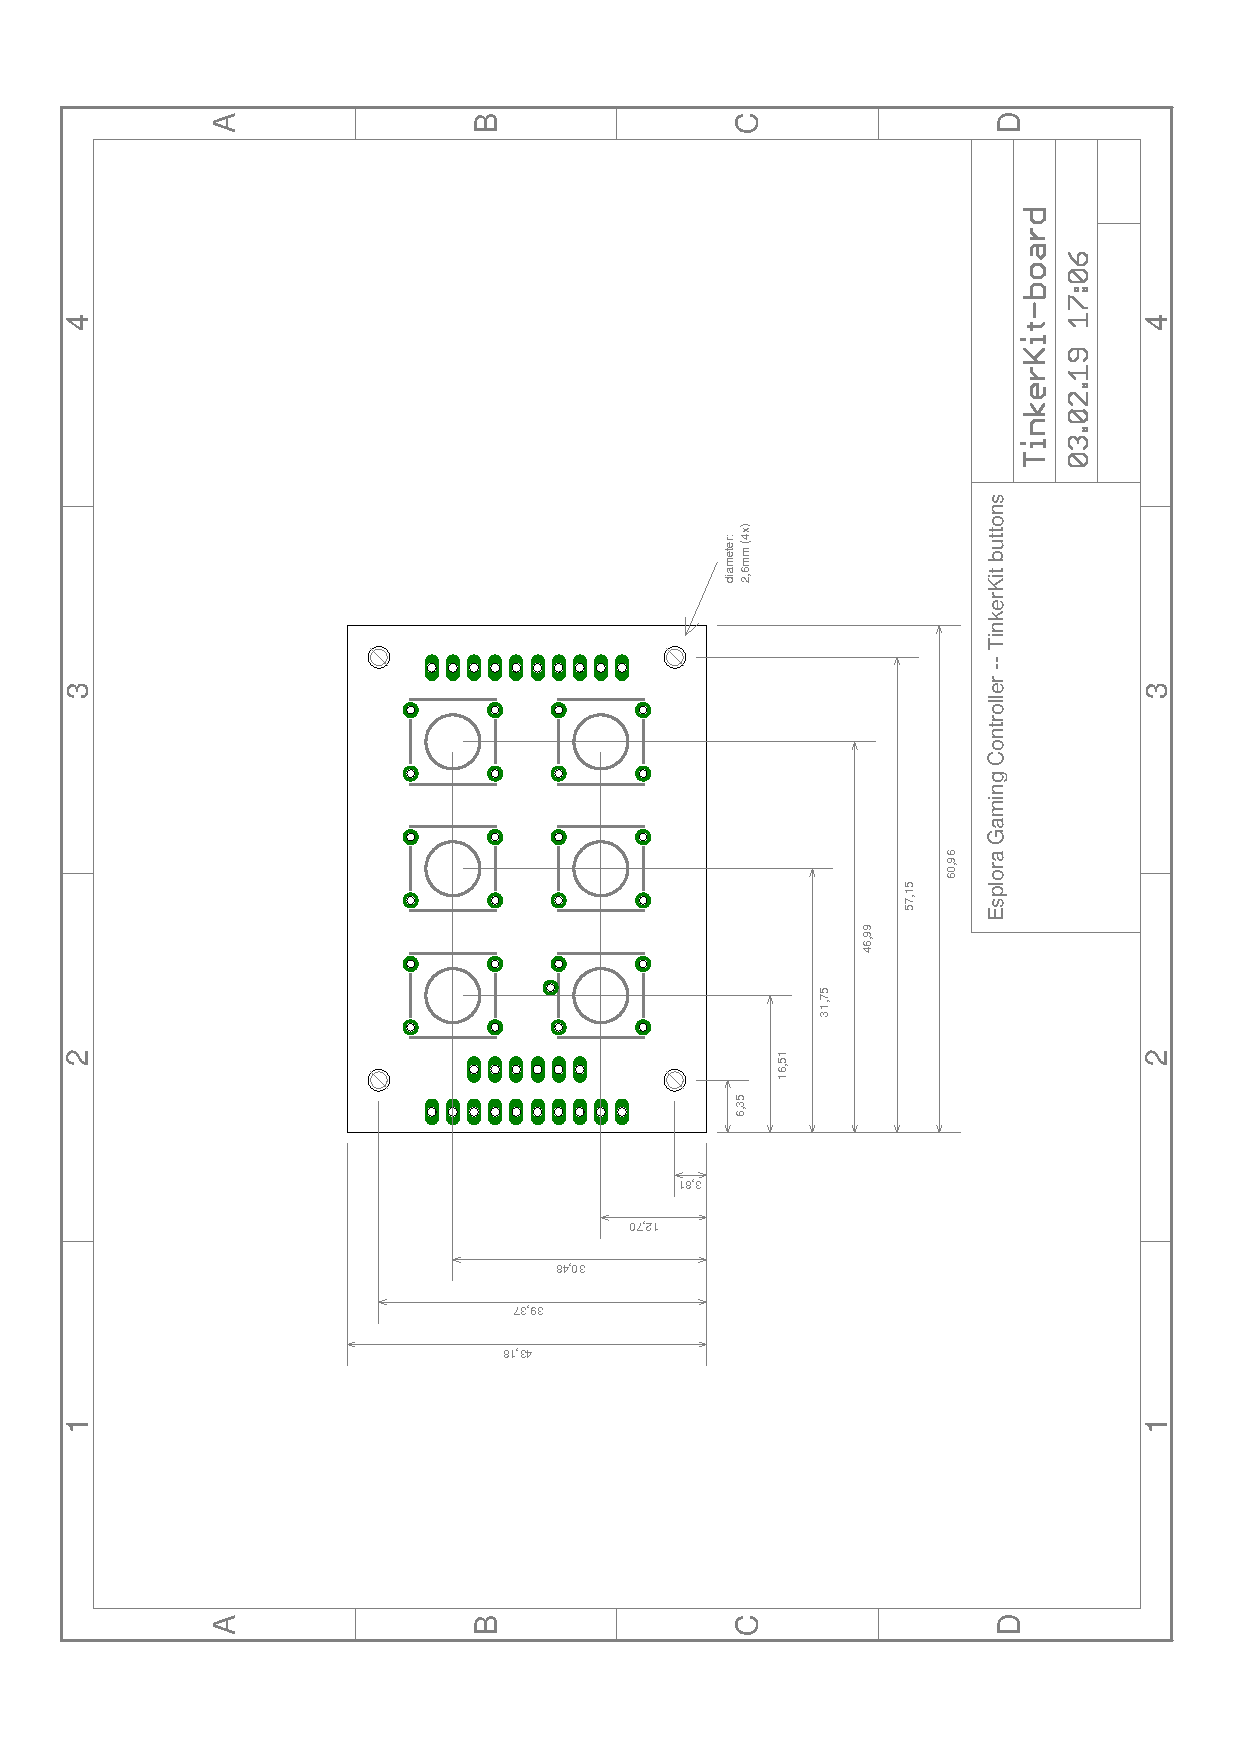
\includepdf[pages=-, , scale=1.0, addtotoc={1,section,0,Zusatzplatine Abmessungen,Zusatzplatine Abmessungen} ]{./pics/eagle/TinkerKit-board_MEAS.pdf}
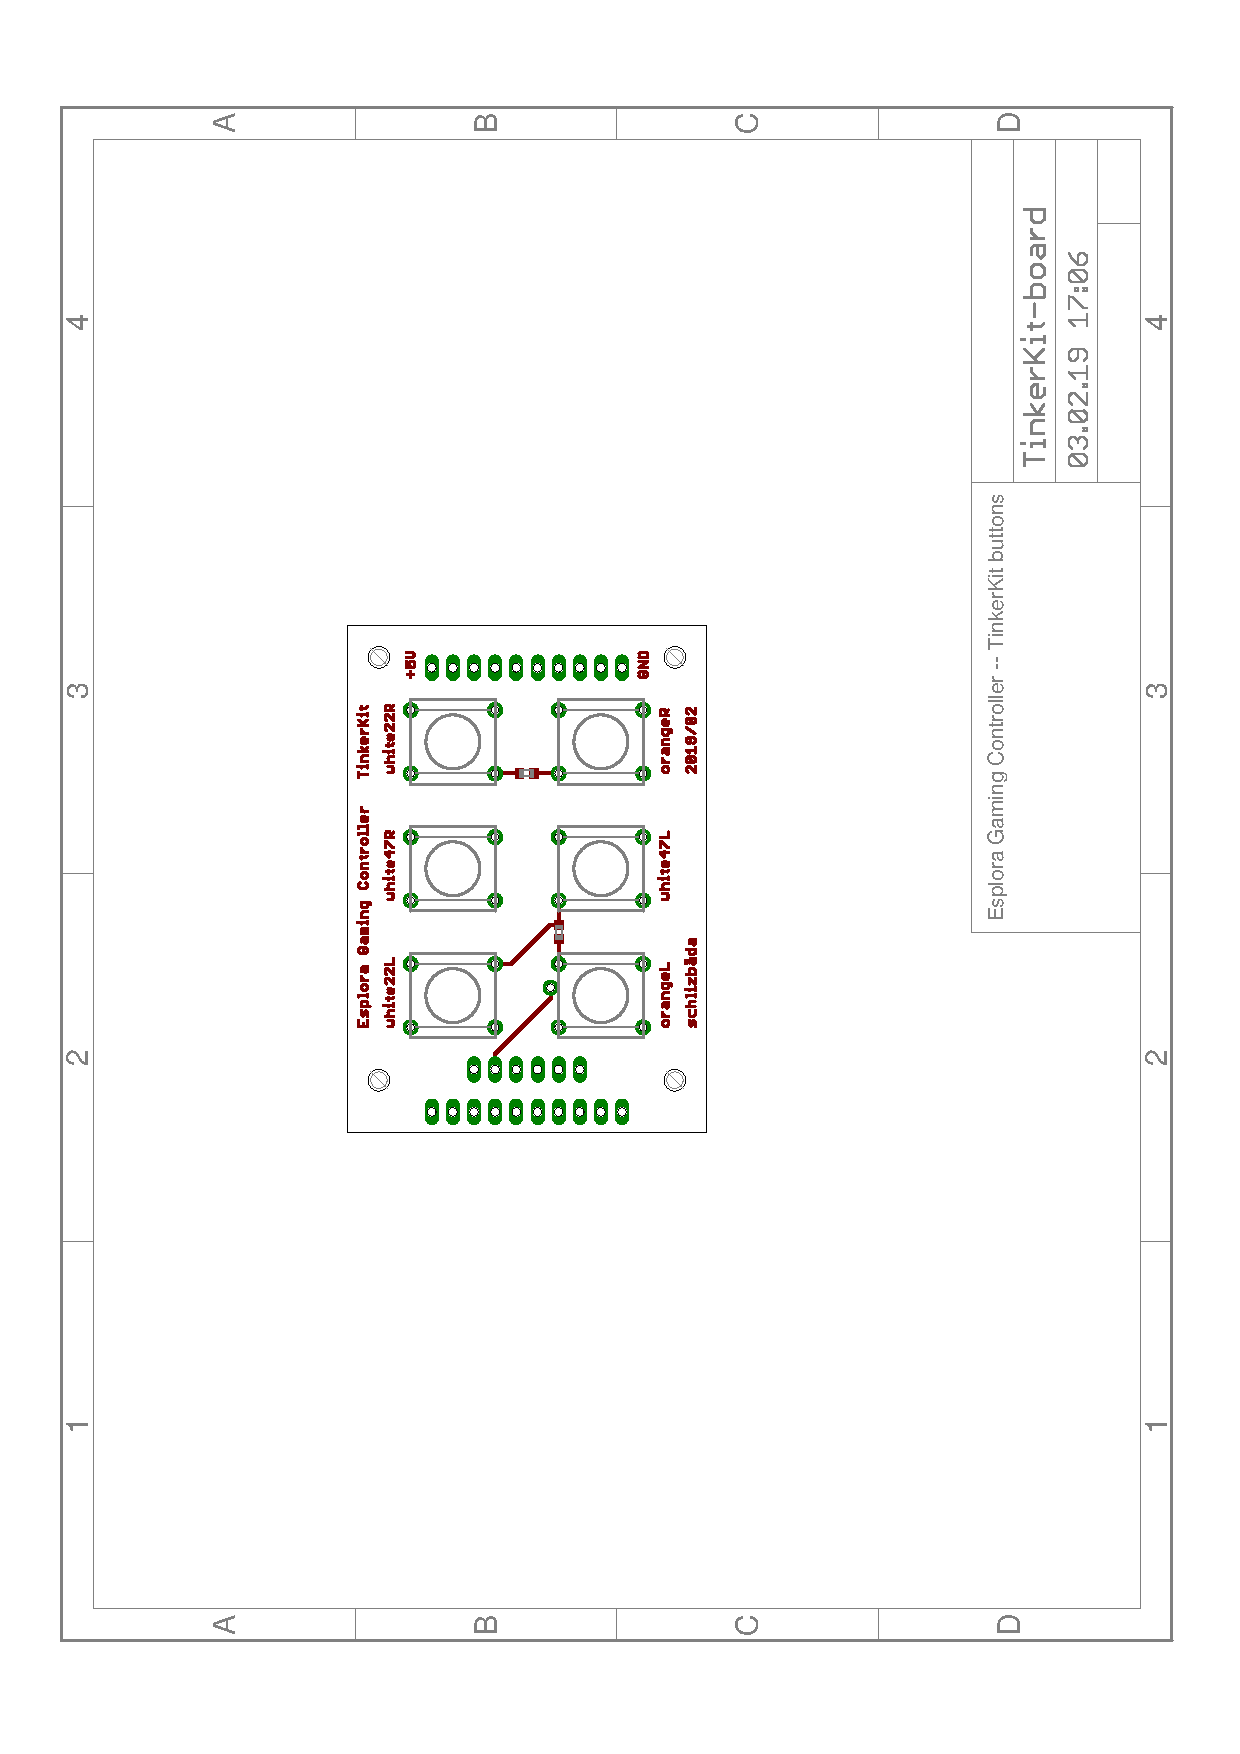
\includepdf[pages=-, , scale=1.0, addtotoc={1,section,0,Zusatzplatine Oberseite,Zusatzplatine Oberseite} ]{./pics/eagle/TinkerKit-board_TOP.pdf}
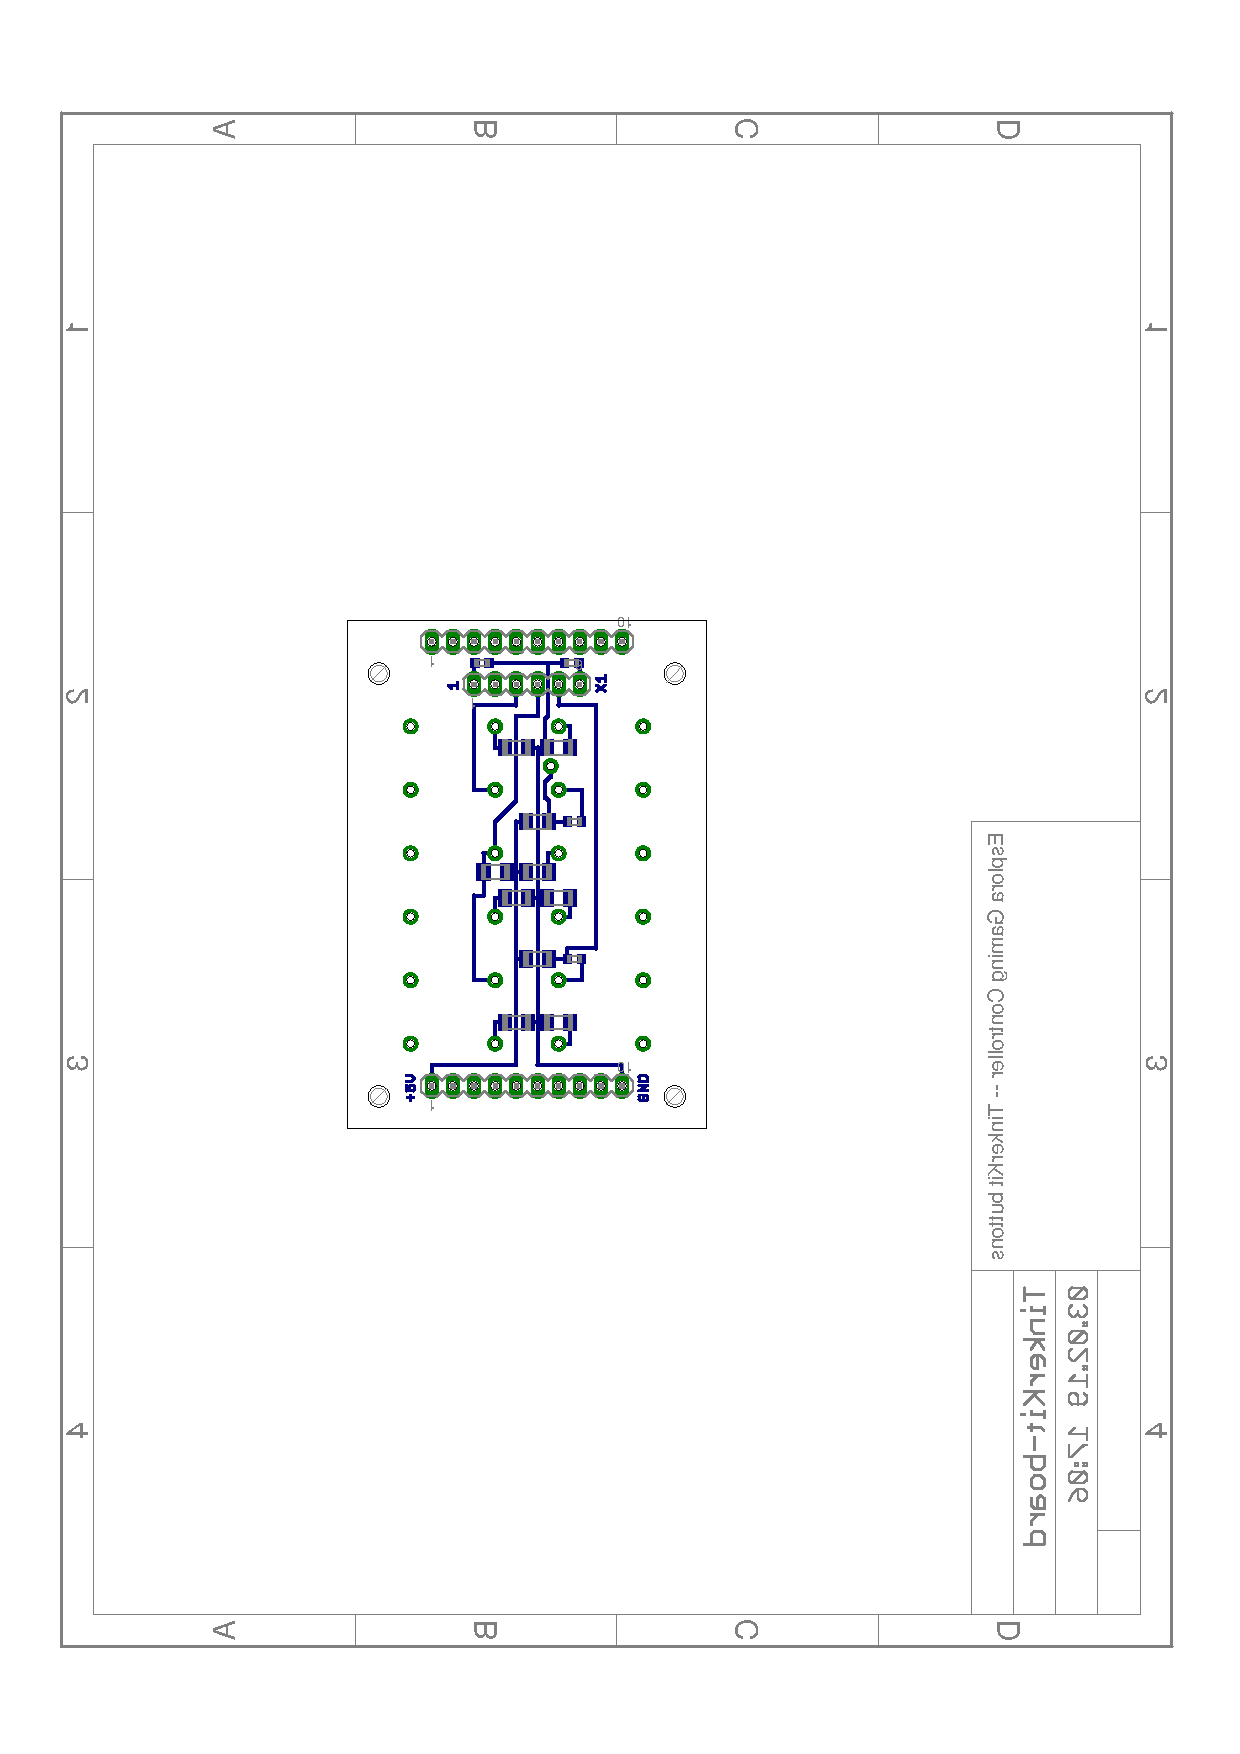
\includepdf[pages=-, , scale=1.0, addtotoc={1,section,0,Zusatzplatine Unterseite,Zusatzplatine Unterseite} ]{./pics/eagle/TinkerKit-board_BOT.pdf}

%%---------------------------------------------------------------
%%  parts
%%---------------------------------------------------------------
%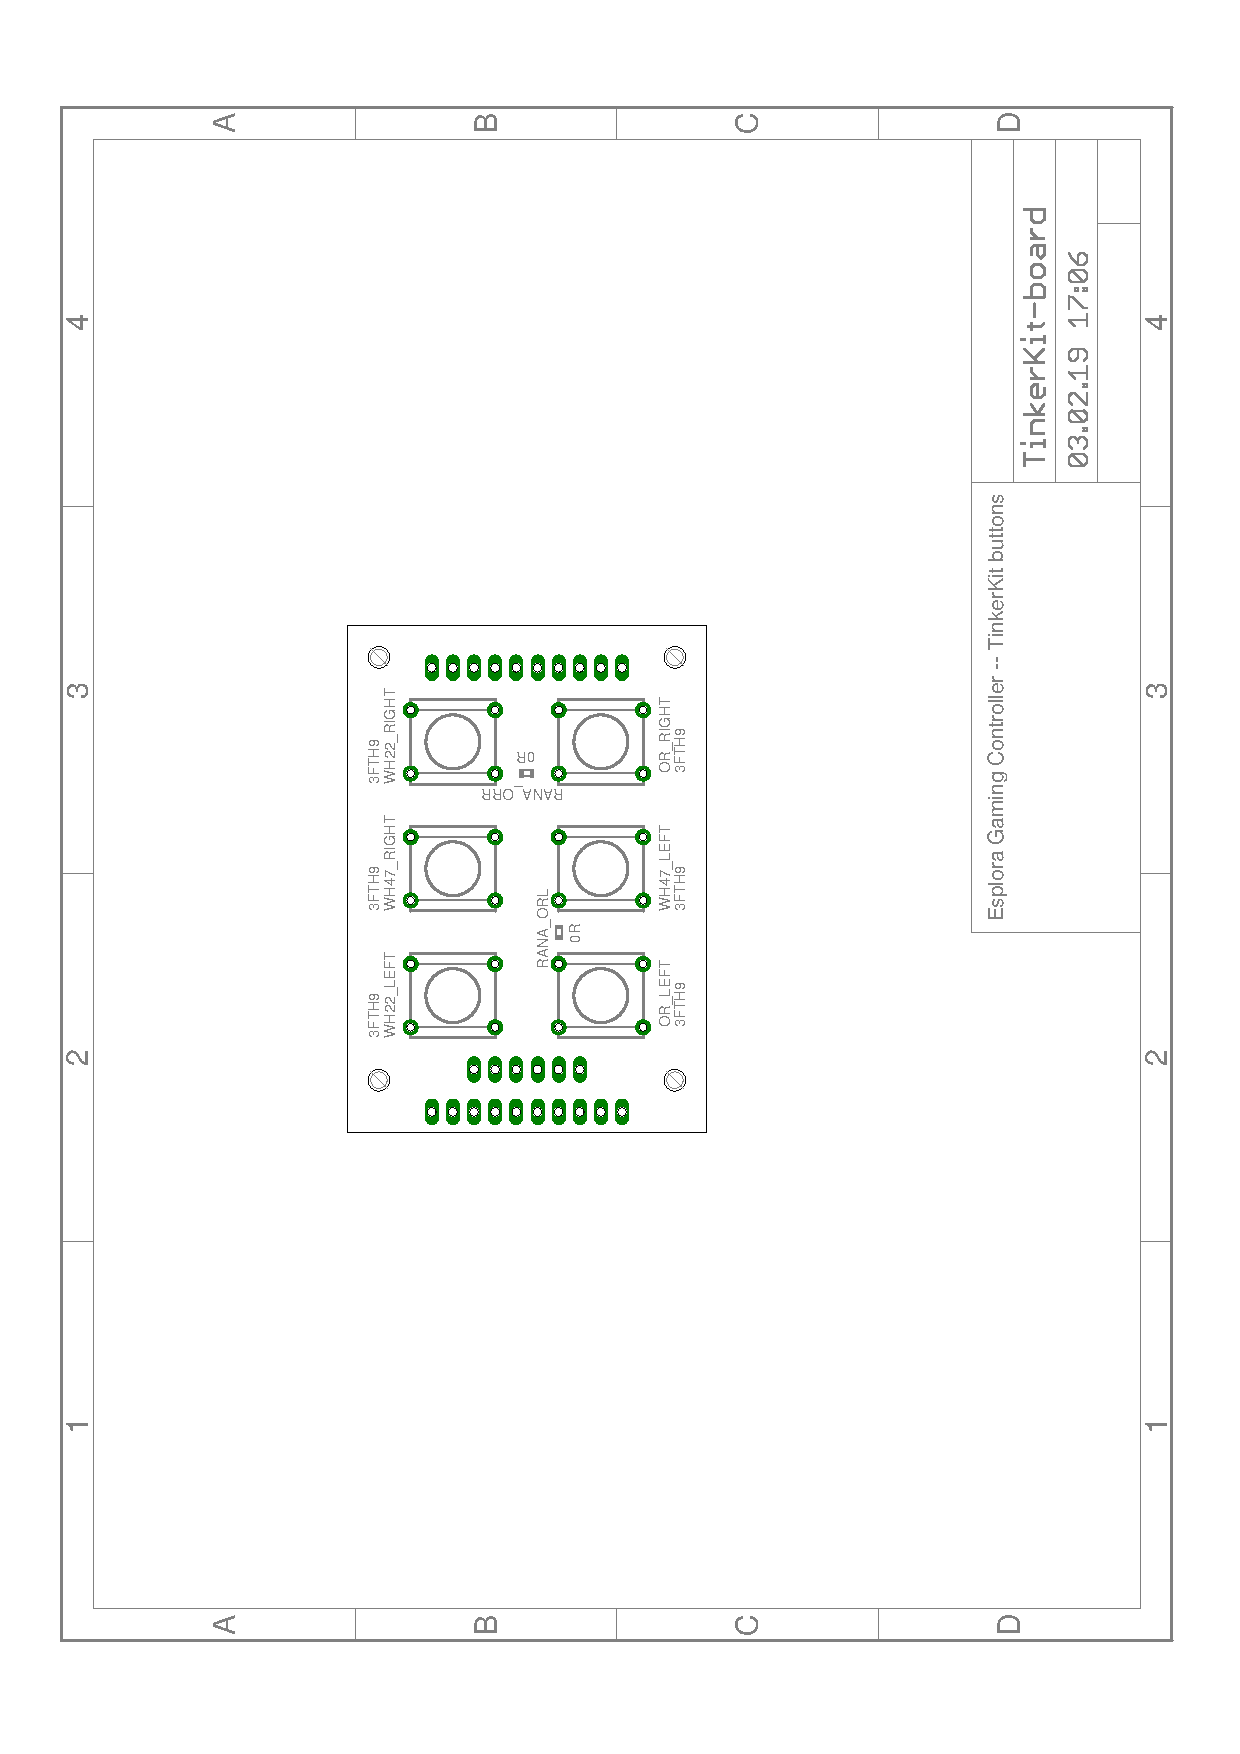
\includepdf[pages=-, , scale=1.0, addtotoc={1,section,0,Leiterplatte,Leiterplatte} ]{./pics/eagle/TinkerKit-board_TOPparts.pdf}
%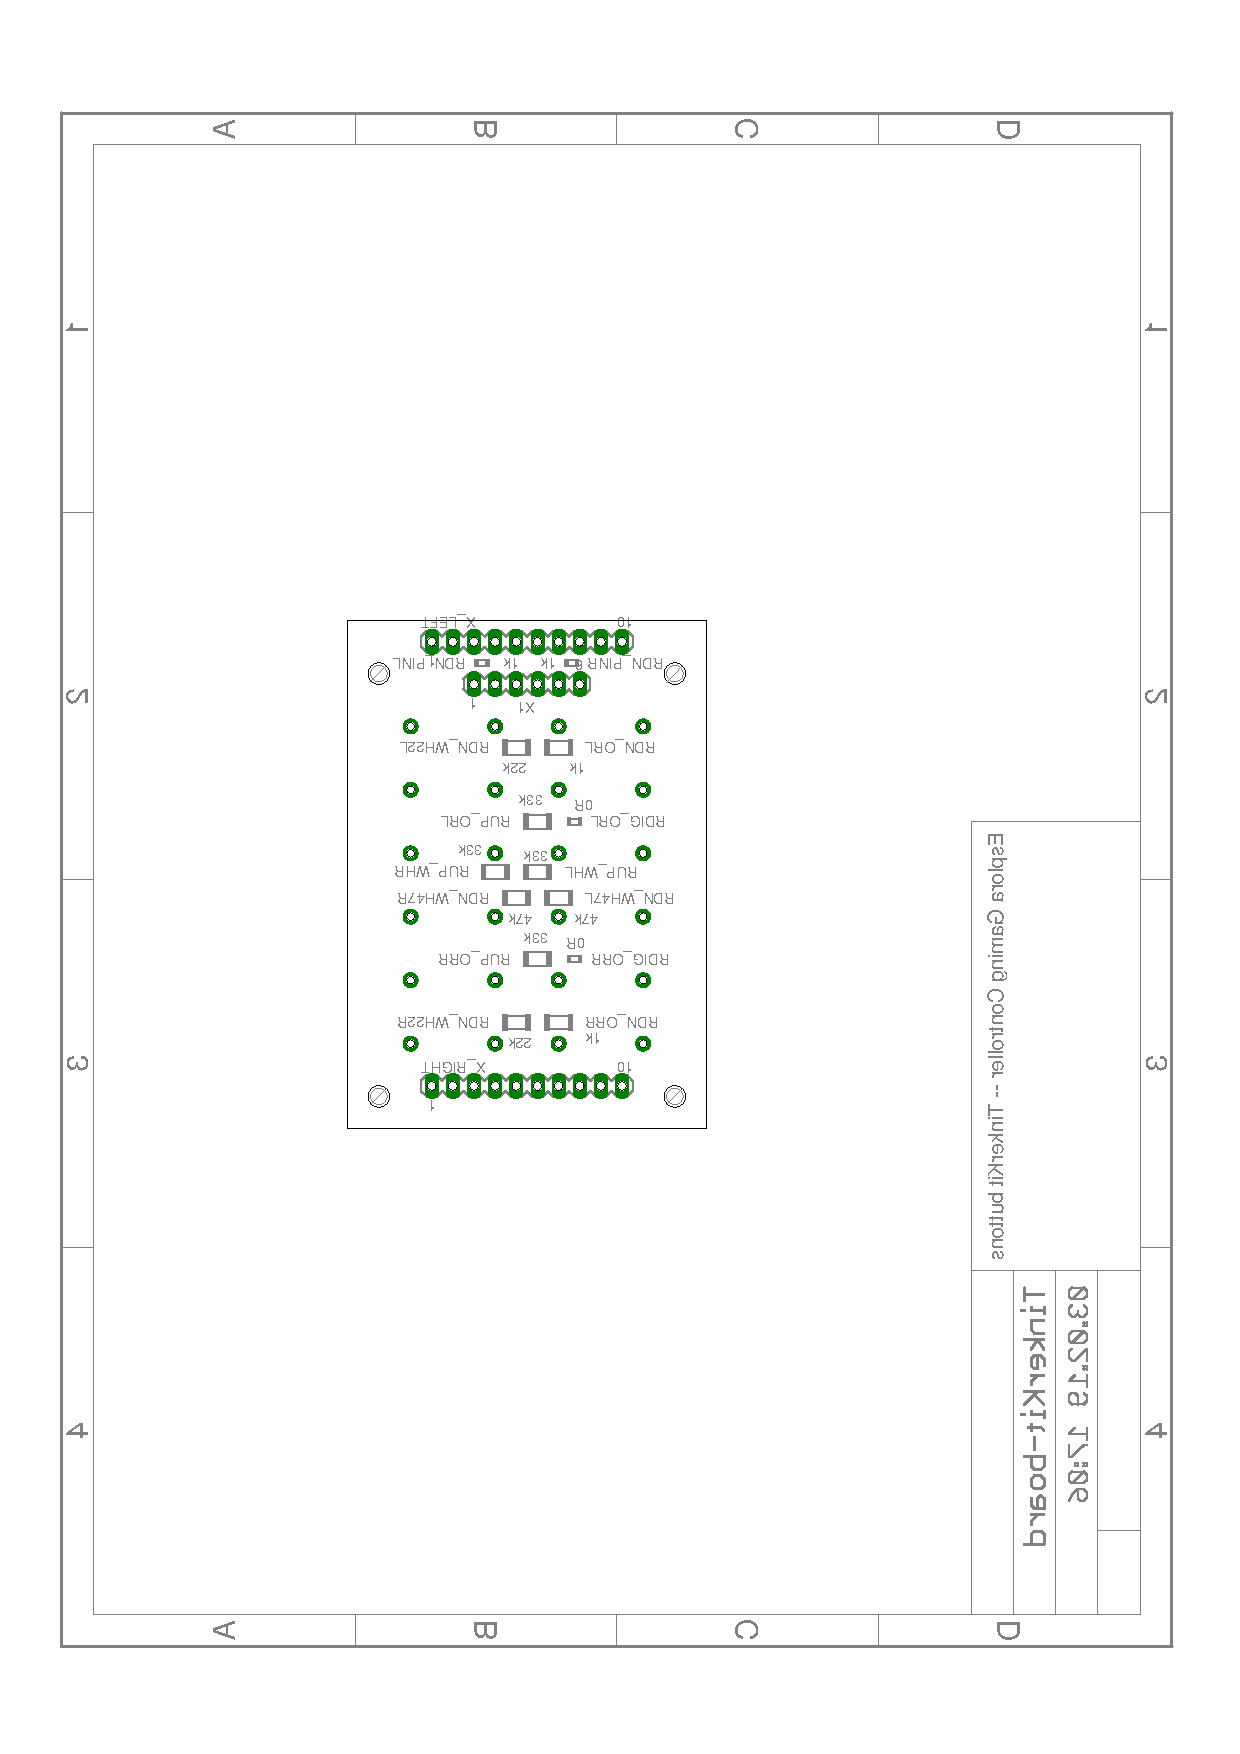
\includepdf[pages=-, , scale=1.0, addtotoc={1,section,0,Leiterplatte,Leiterplatte} ]{./pics/eagle/TinkerKit-board_BOTparts.pdf}

\end{appendix}

% Index ------------------------------------------------------------------------
%   activate the following line to add an index.
% ------------------------------------------------------------------------------
%\printindex

\end{document}
